%!TEX program = xelatex

\documentclass[13pt, final]{beamer}
\usepackage{amsmath}
\usepackage{mathtools}
\usepackage{graphbox}
\usepackage{color}
\usepackage{todonotes}
\usepackage[export]{adjustbox}

\setbeamercovered{transparent=60}

\usepackage[backend=bibtex]{biblatex}
\bibliography{biblio}
\nocite{*}

% \usepackage[compatibility=false]{caption}
% \usepackage{subcaption}


\setbeamercovered{dynamic}

% Beamer settings
\usetheme{metropolis}
\metroset{
	everytitleformat=uppercase,
	progressbar=frametitle
} 

\renewcommand{\vec}[1]{\boldsymbol{#1}}
\newcommand{\hsp}{\hspace{0.5em}}

\title{Point Normal triangles}
\author{Rick van Veen \and Laura Baakman}
\date{December 14, 2015}
\institute{Advanced Computer Graphics}

\begin{document}
	\begin{frame}
		\titlepage
	\end{frame}

	% \section{Introduction}
	% !TEX root = presentation.tex
% \begin{frame}
%     \frametitle{Minkowski Sum}
%     \framesubtitle{Example}
%     \topskip0pt
% 	\vspace*{\fill}
%     \begin{center}
%     	\todo[inline]{Schermvullend plaatje}
% 	\end{center}
% 	\vspace*{\fill}
% 	\mbox{\tiny{Image adapted from: \url{http://allenchou.net/2013/12/game-physics-collision-detection-csos-support-functions/}}}
% \end{frame}

\plain{	
	\begin{columns}
		\begin{column}[b]{.25\textwidth}
			\begin{center}
			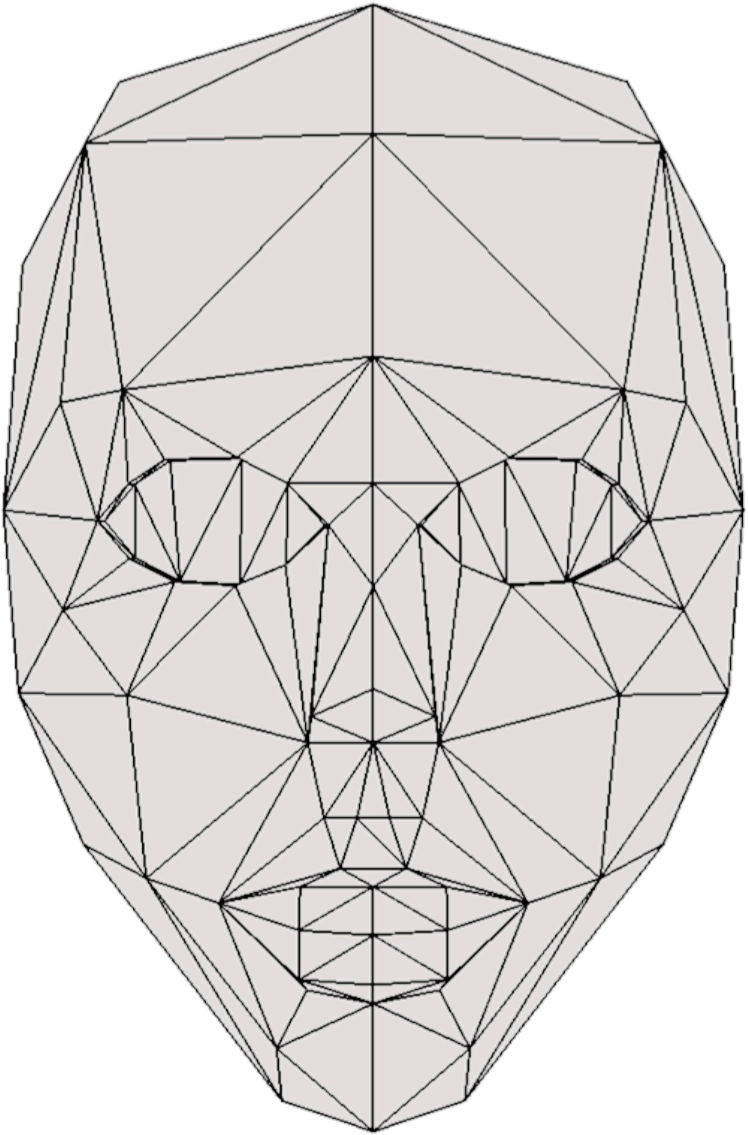
\includegraphics[width=\textwidth]{./img/0_intro/00_results_orange_1.png}
			 \small{input mesh}
			\end{center}
		\end{column}
		\begin{column}[b]{.25\textwidth}
			\begin{center}
			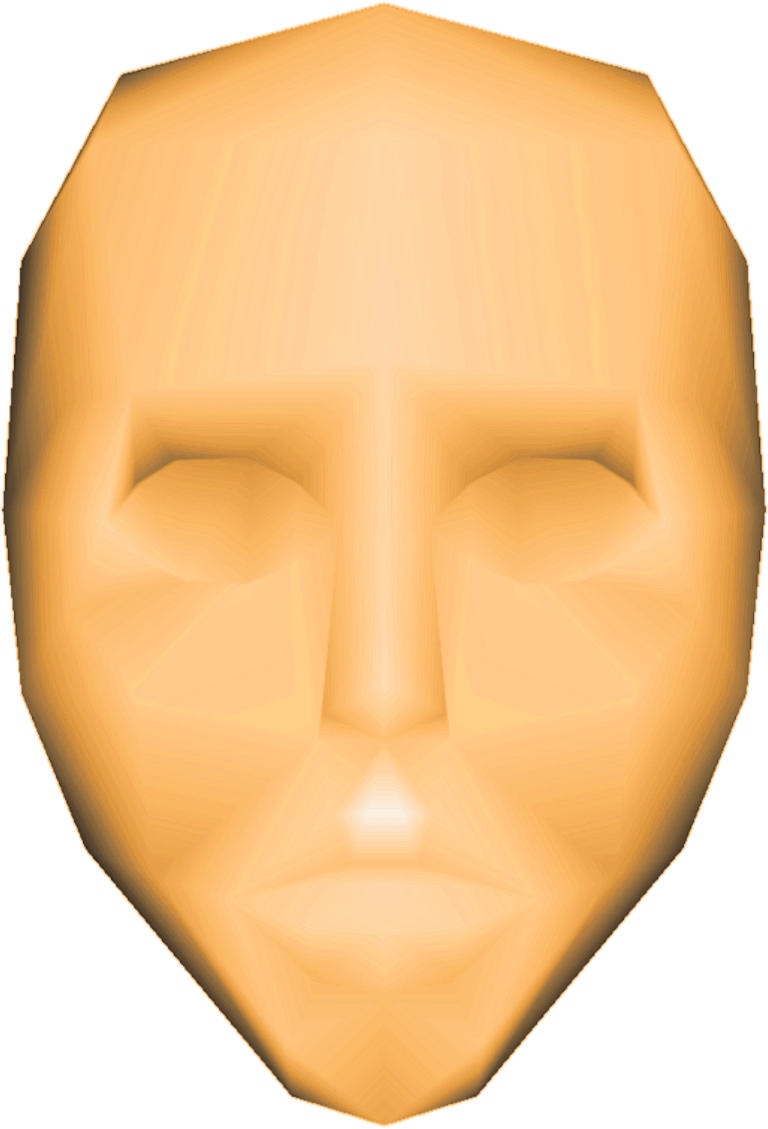
\includegraphics[width=\textwidth]{./img/0_intro/00_results_orange_2.png}
			\small{gouraud}
			\end{center}
		\end{column}
		\begin{column}[b]{.25\textwidth}
			\begin{center}
			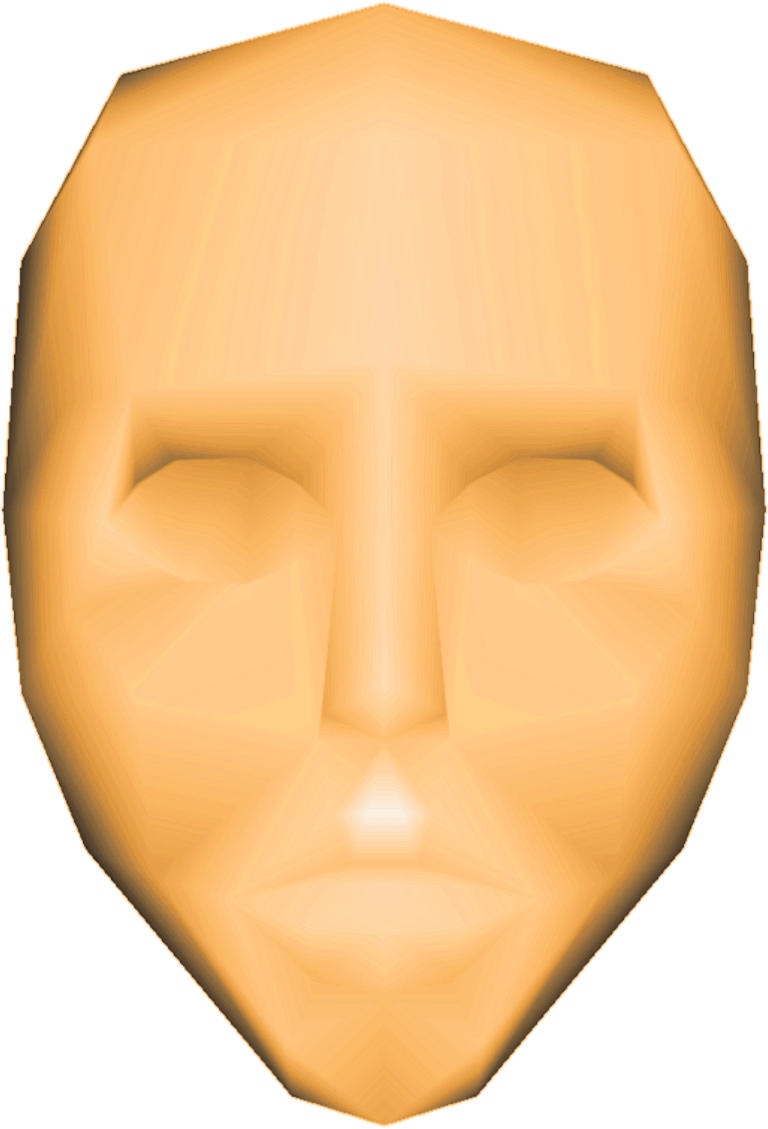
\includegraphics[width=\textwidth]{./img/0_intro/00_results_orange_3.png}
			\small{pn geometry}
			\end{center}
		\end{column}
		\begin{column}[b]{.25\textwidth}
			\begin{center}
			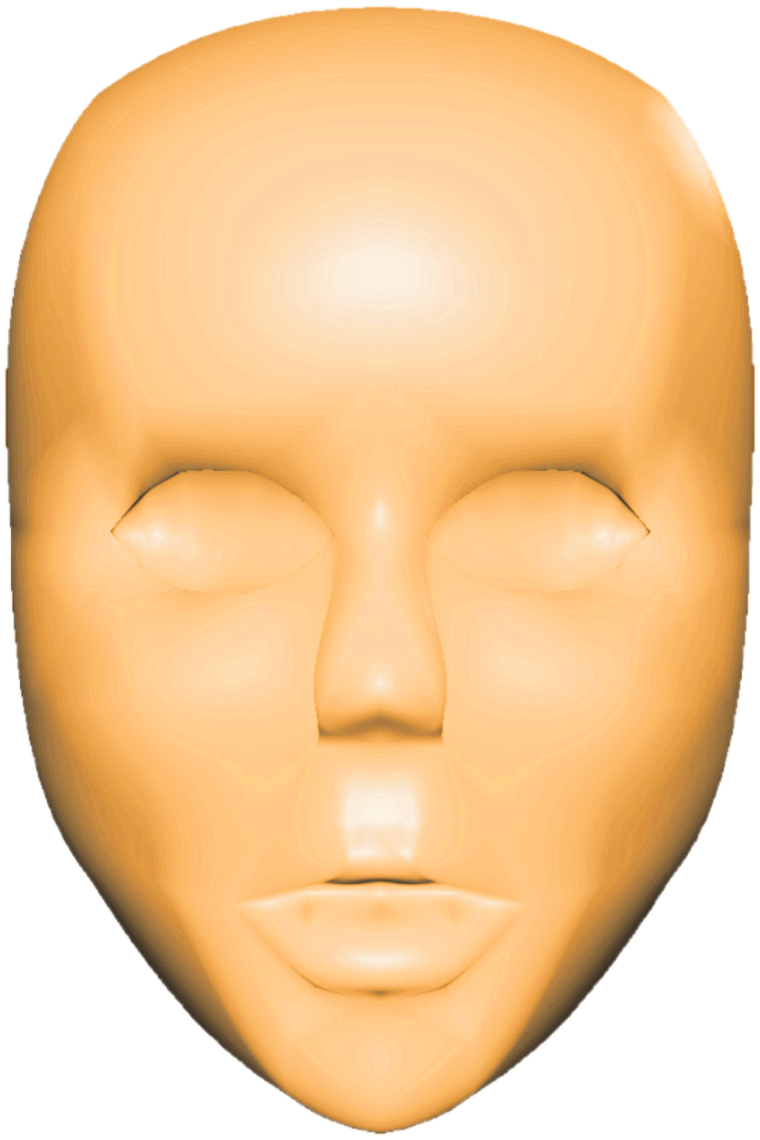
\includegraphics[width=\textwidth]{./img/0_intro/00_results_orange_4.png}
			\small{pn triangles}
			\end{center}
		\end{column}
	\end{columns}
	
	\note{\textbf{[Rick]}}
	\note[item]{Tell what can be seen on the slide.}
	\note[item]{Stand still by the geometry}
	\note[item]{PN triangle -> more \textbf{organic shapes} (and \textbf{continuous surface})}
	\note[item]{Relatively easy to extend existing `pipeline'}
}


	\section{Single PN Triangle}
	% !TEX root = presentation.tex
	\begin{frame}\frametitle{Cubic B\'ezier triangles}
		\begin{columns}
			\begin{column}{0.6\textwidth}
				\todo[inline]{What are they.}
			\end{column}
		\end{columns}
	\end{frame}

	\begin{frame}\frametitle{Geometry}
		\begin{columns}
			\begin{column}{0.6\textwidth}
				\begin{center}
					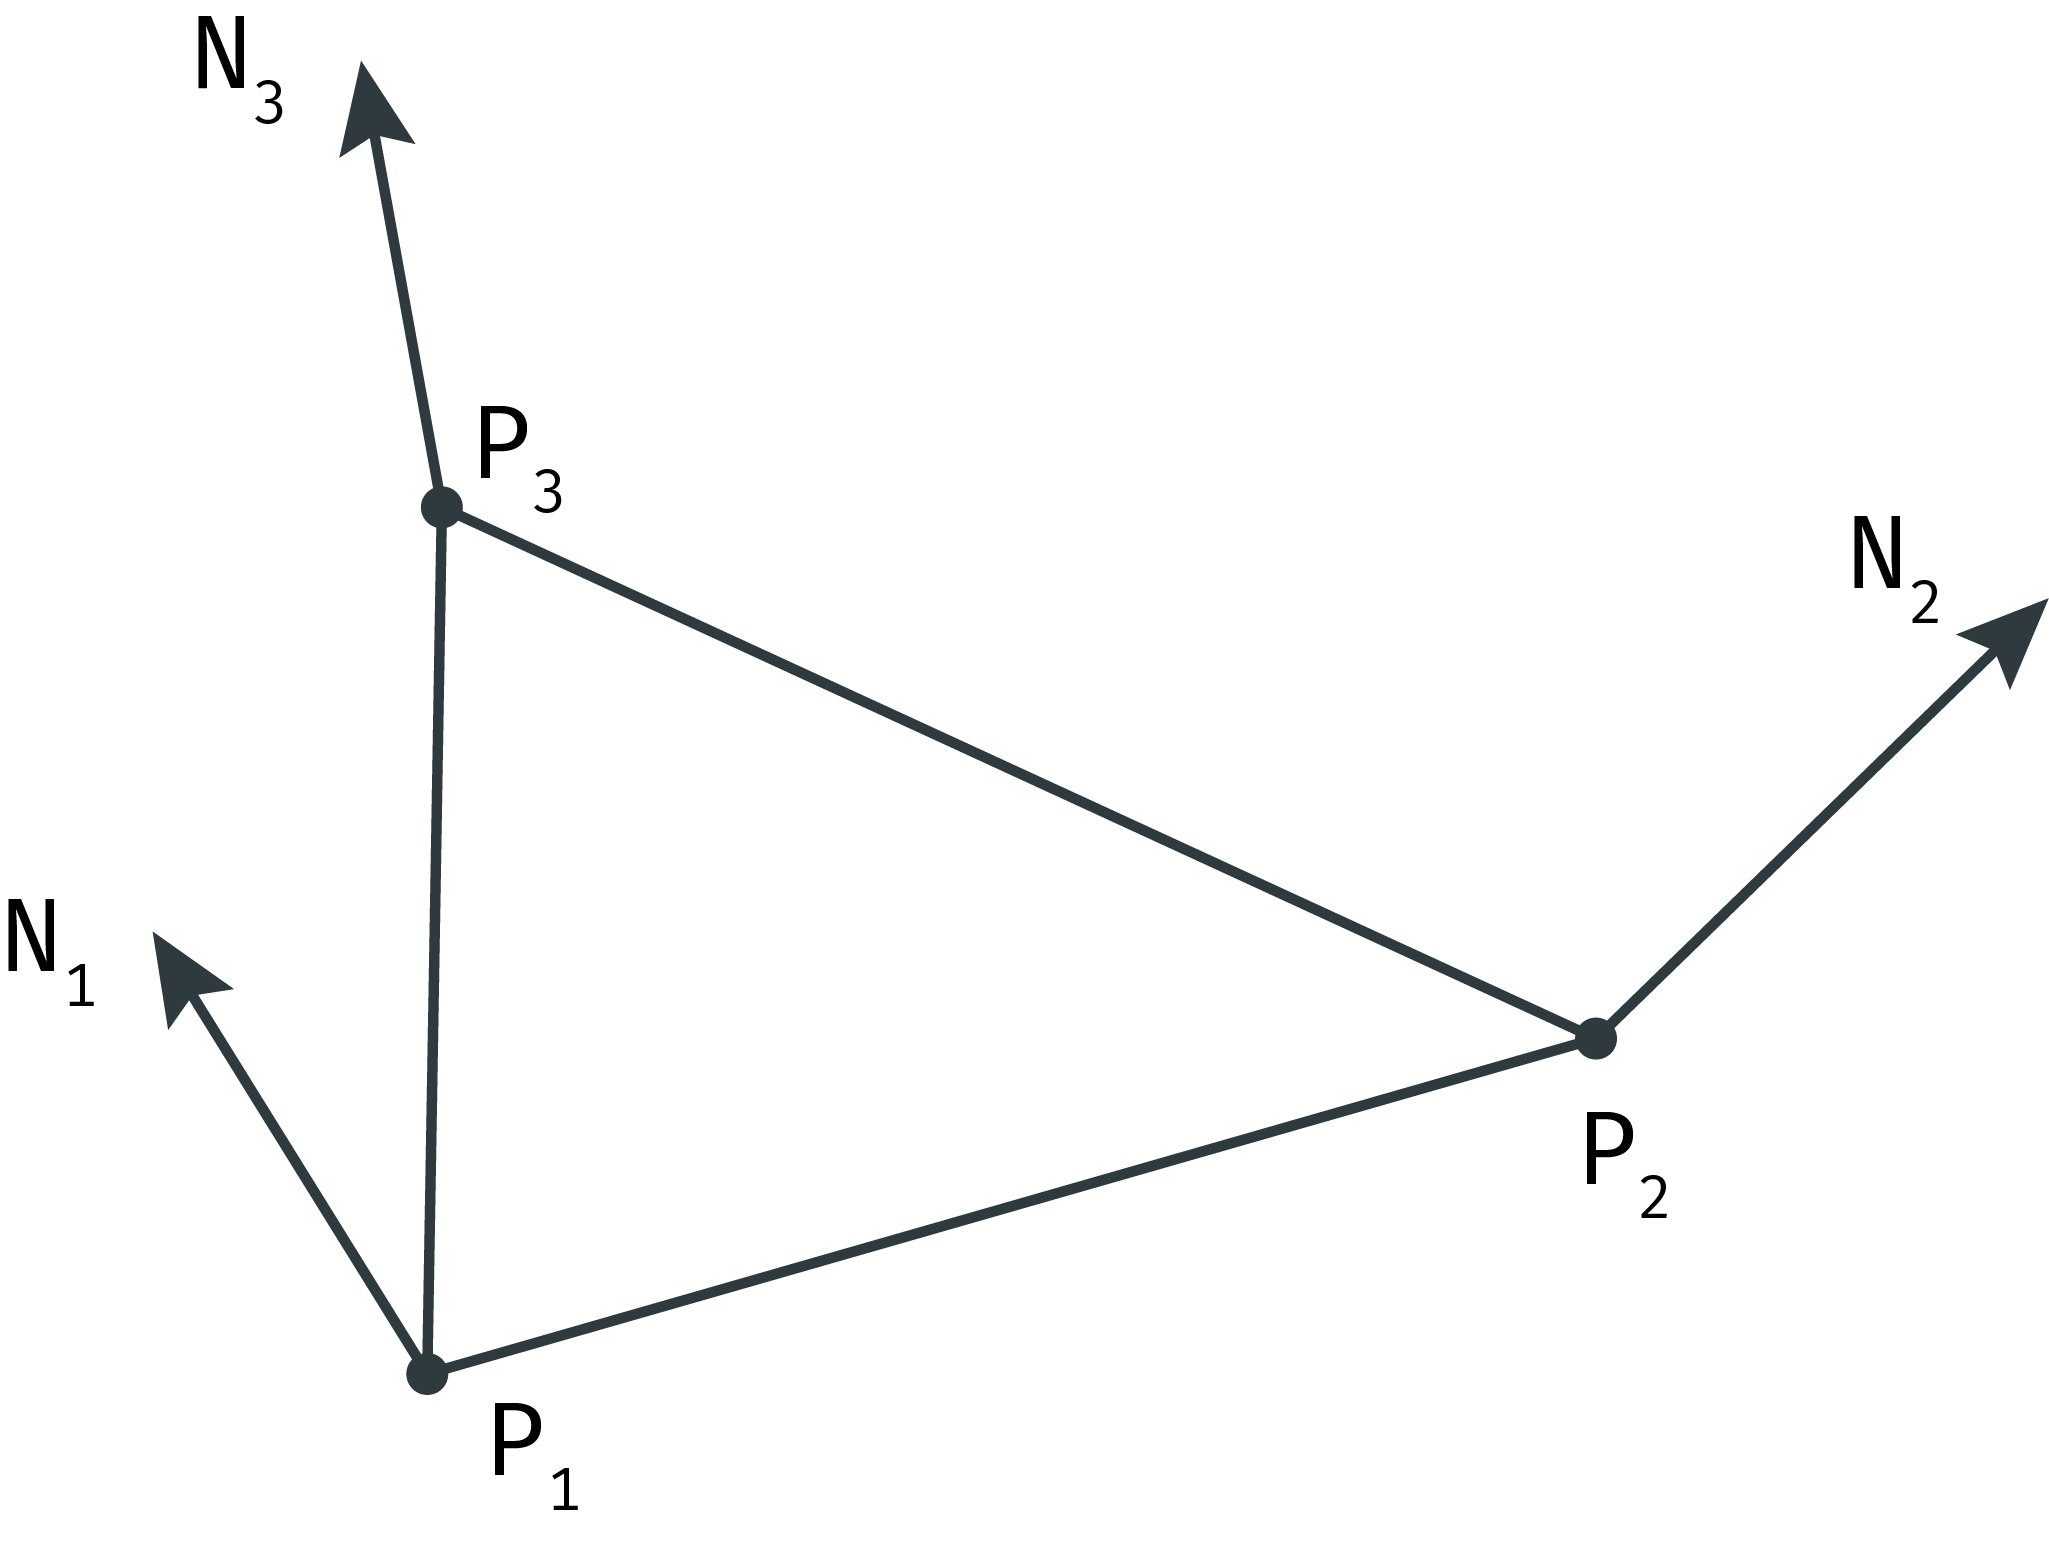
\includegraphics[width=\textwidth]{img/1_single/inputPrimitive.png}
					\small{Input primitive}
				\end{center}
			\end{column}
		\end{columns}
	\end{frame}

	% Geometry process
	\begin{frame}\frametitle{Geometry - step 1}
		\begin{columns}
			\begin{column}{0.6\textwidth}
				\begin{center}
					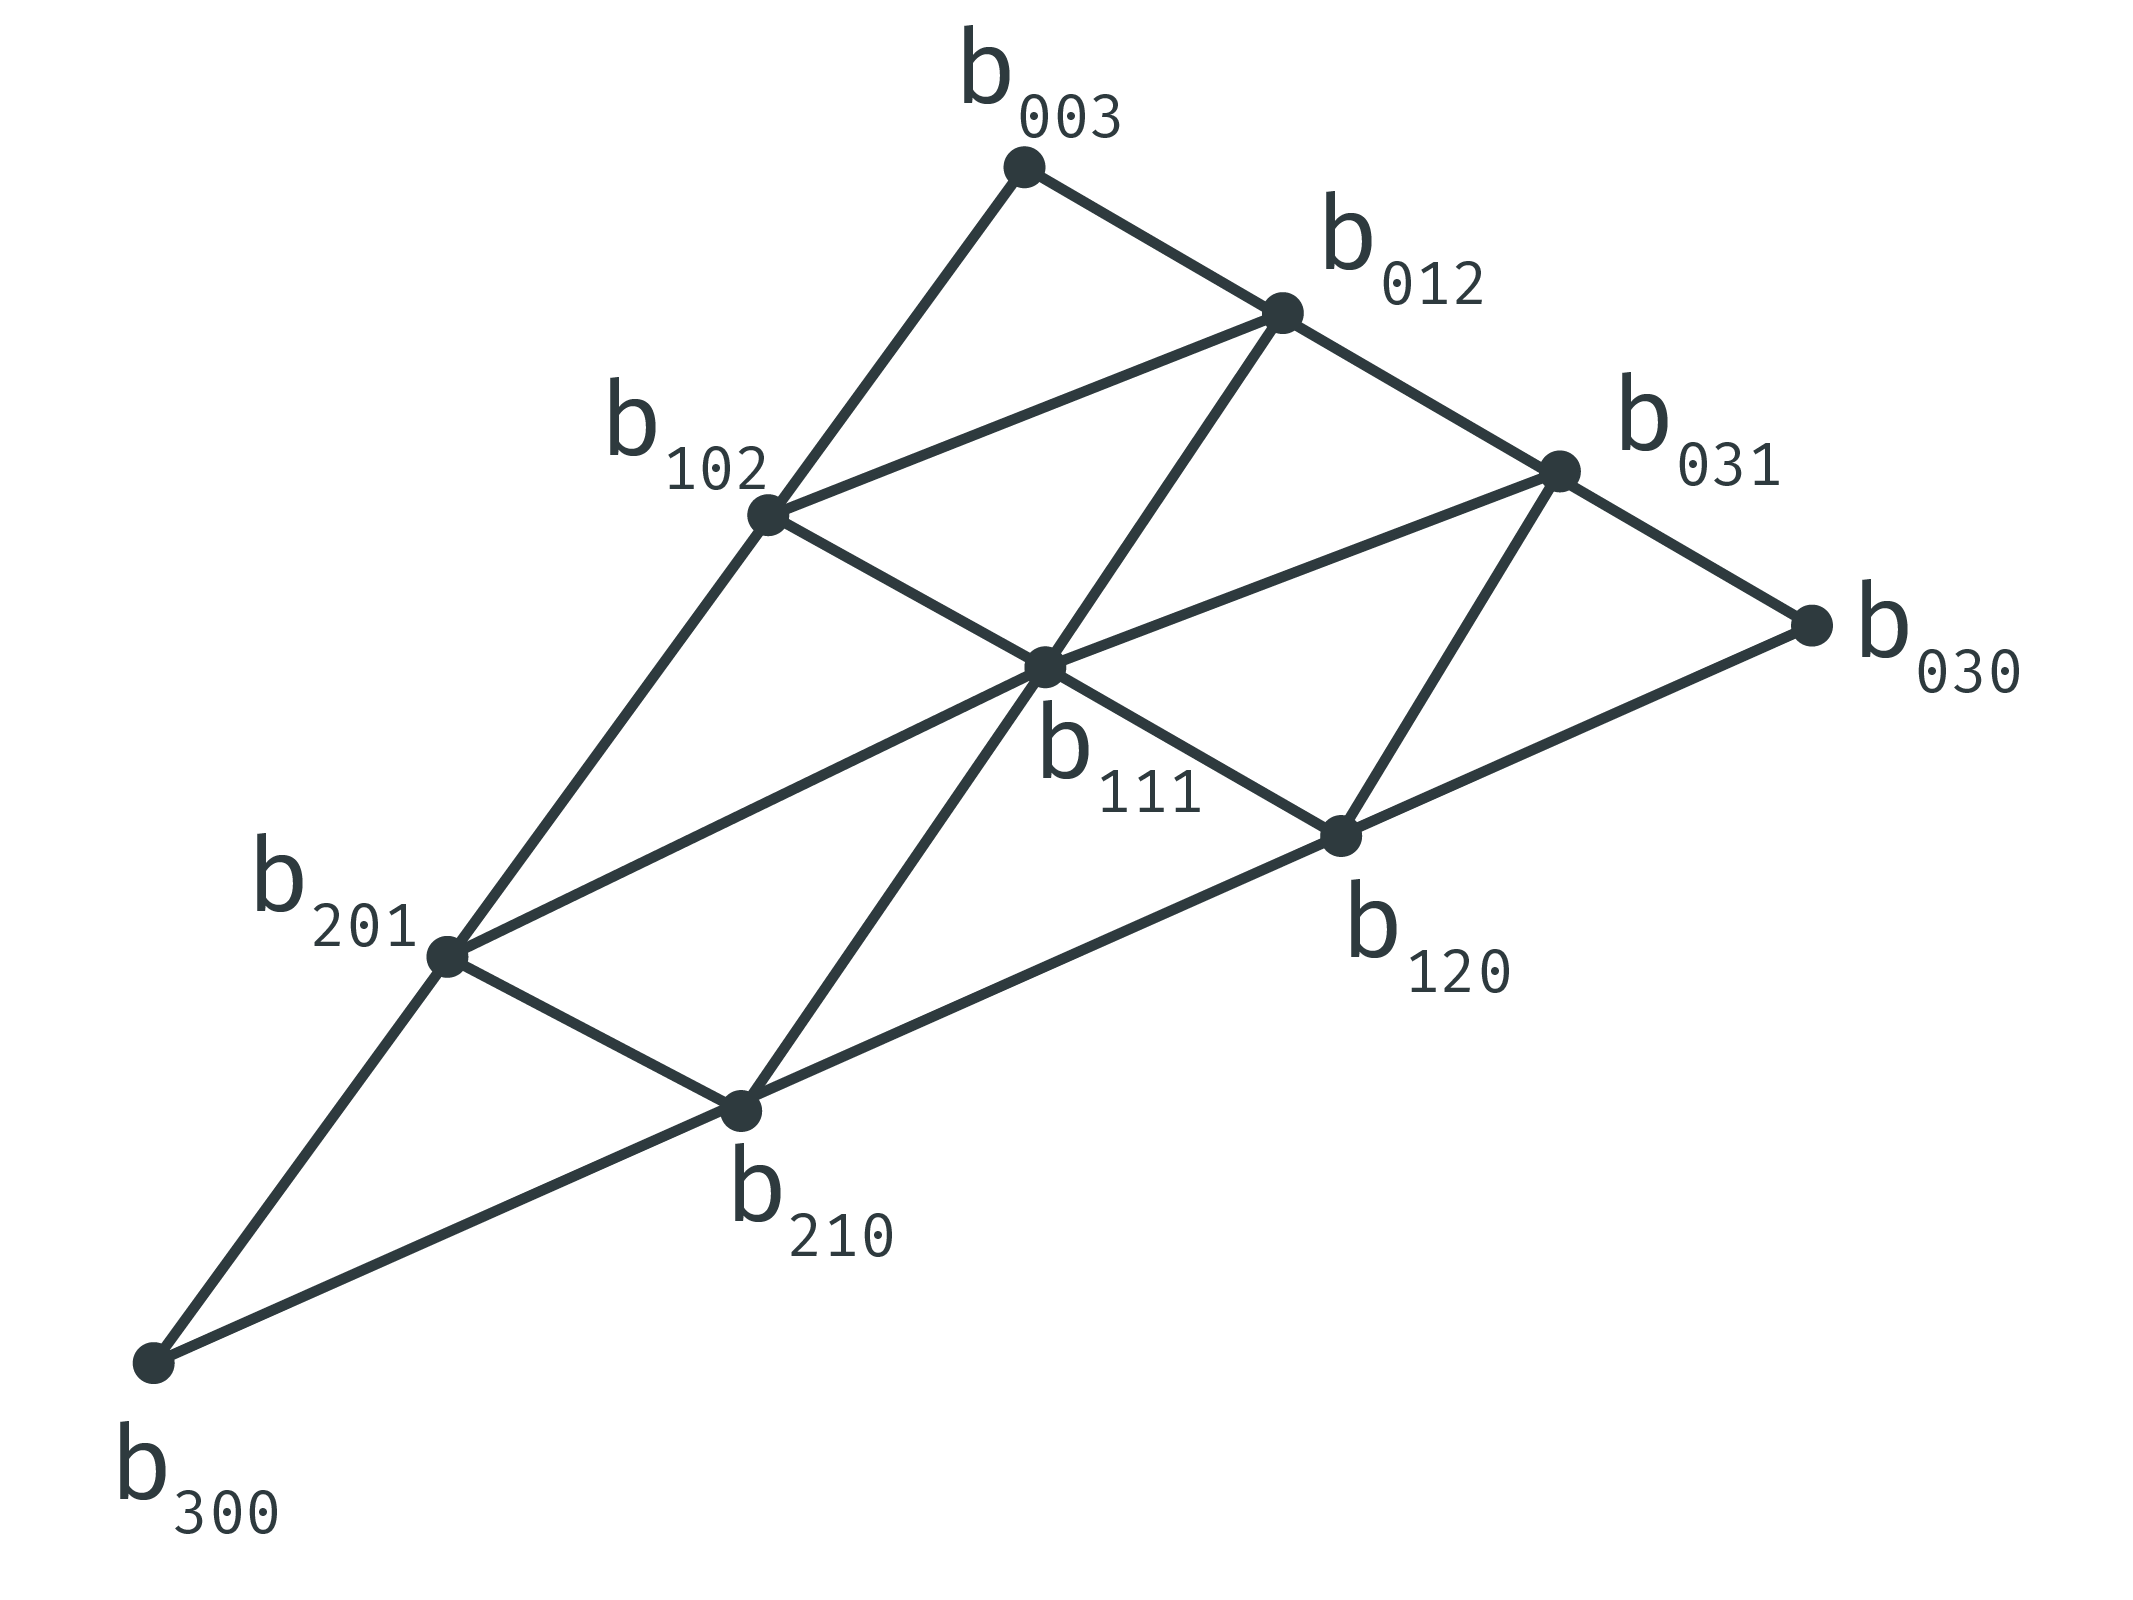
\includegraphics[width=\textwidth]{img/1_single/geometry_1.png}
					\small{Control net}
				\end{center}
			\end{column}
			\uncover<2>{
				\begin{column}{0.4\textwidth}
					\begin{equation*}
						b_{ijk} = (iP_1 + jP_2 + kP_3)/3
					\end{equation*}
				\end{column}
			}
		\end{columns}
	\end{frame}

	\begin{frame}\frametitle{Geometry - step 2}
		\begin{columns}
			\begin{column}{0.6\textwidth}
				\begin{center}
				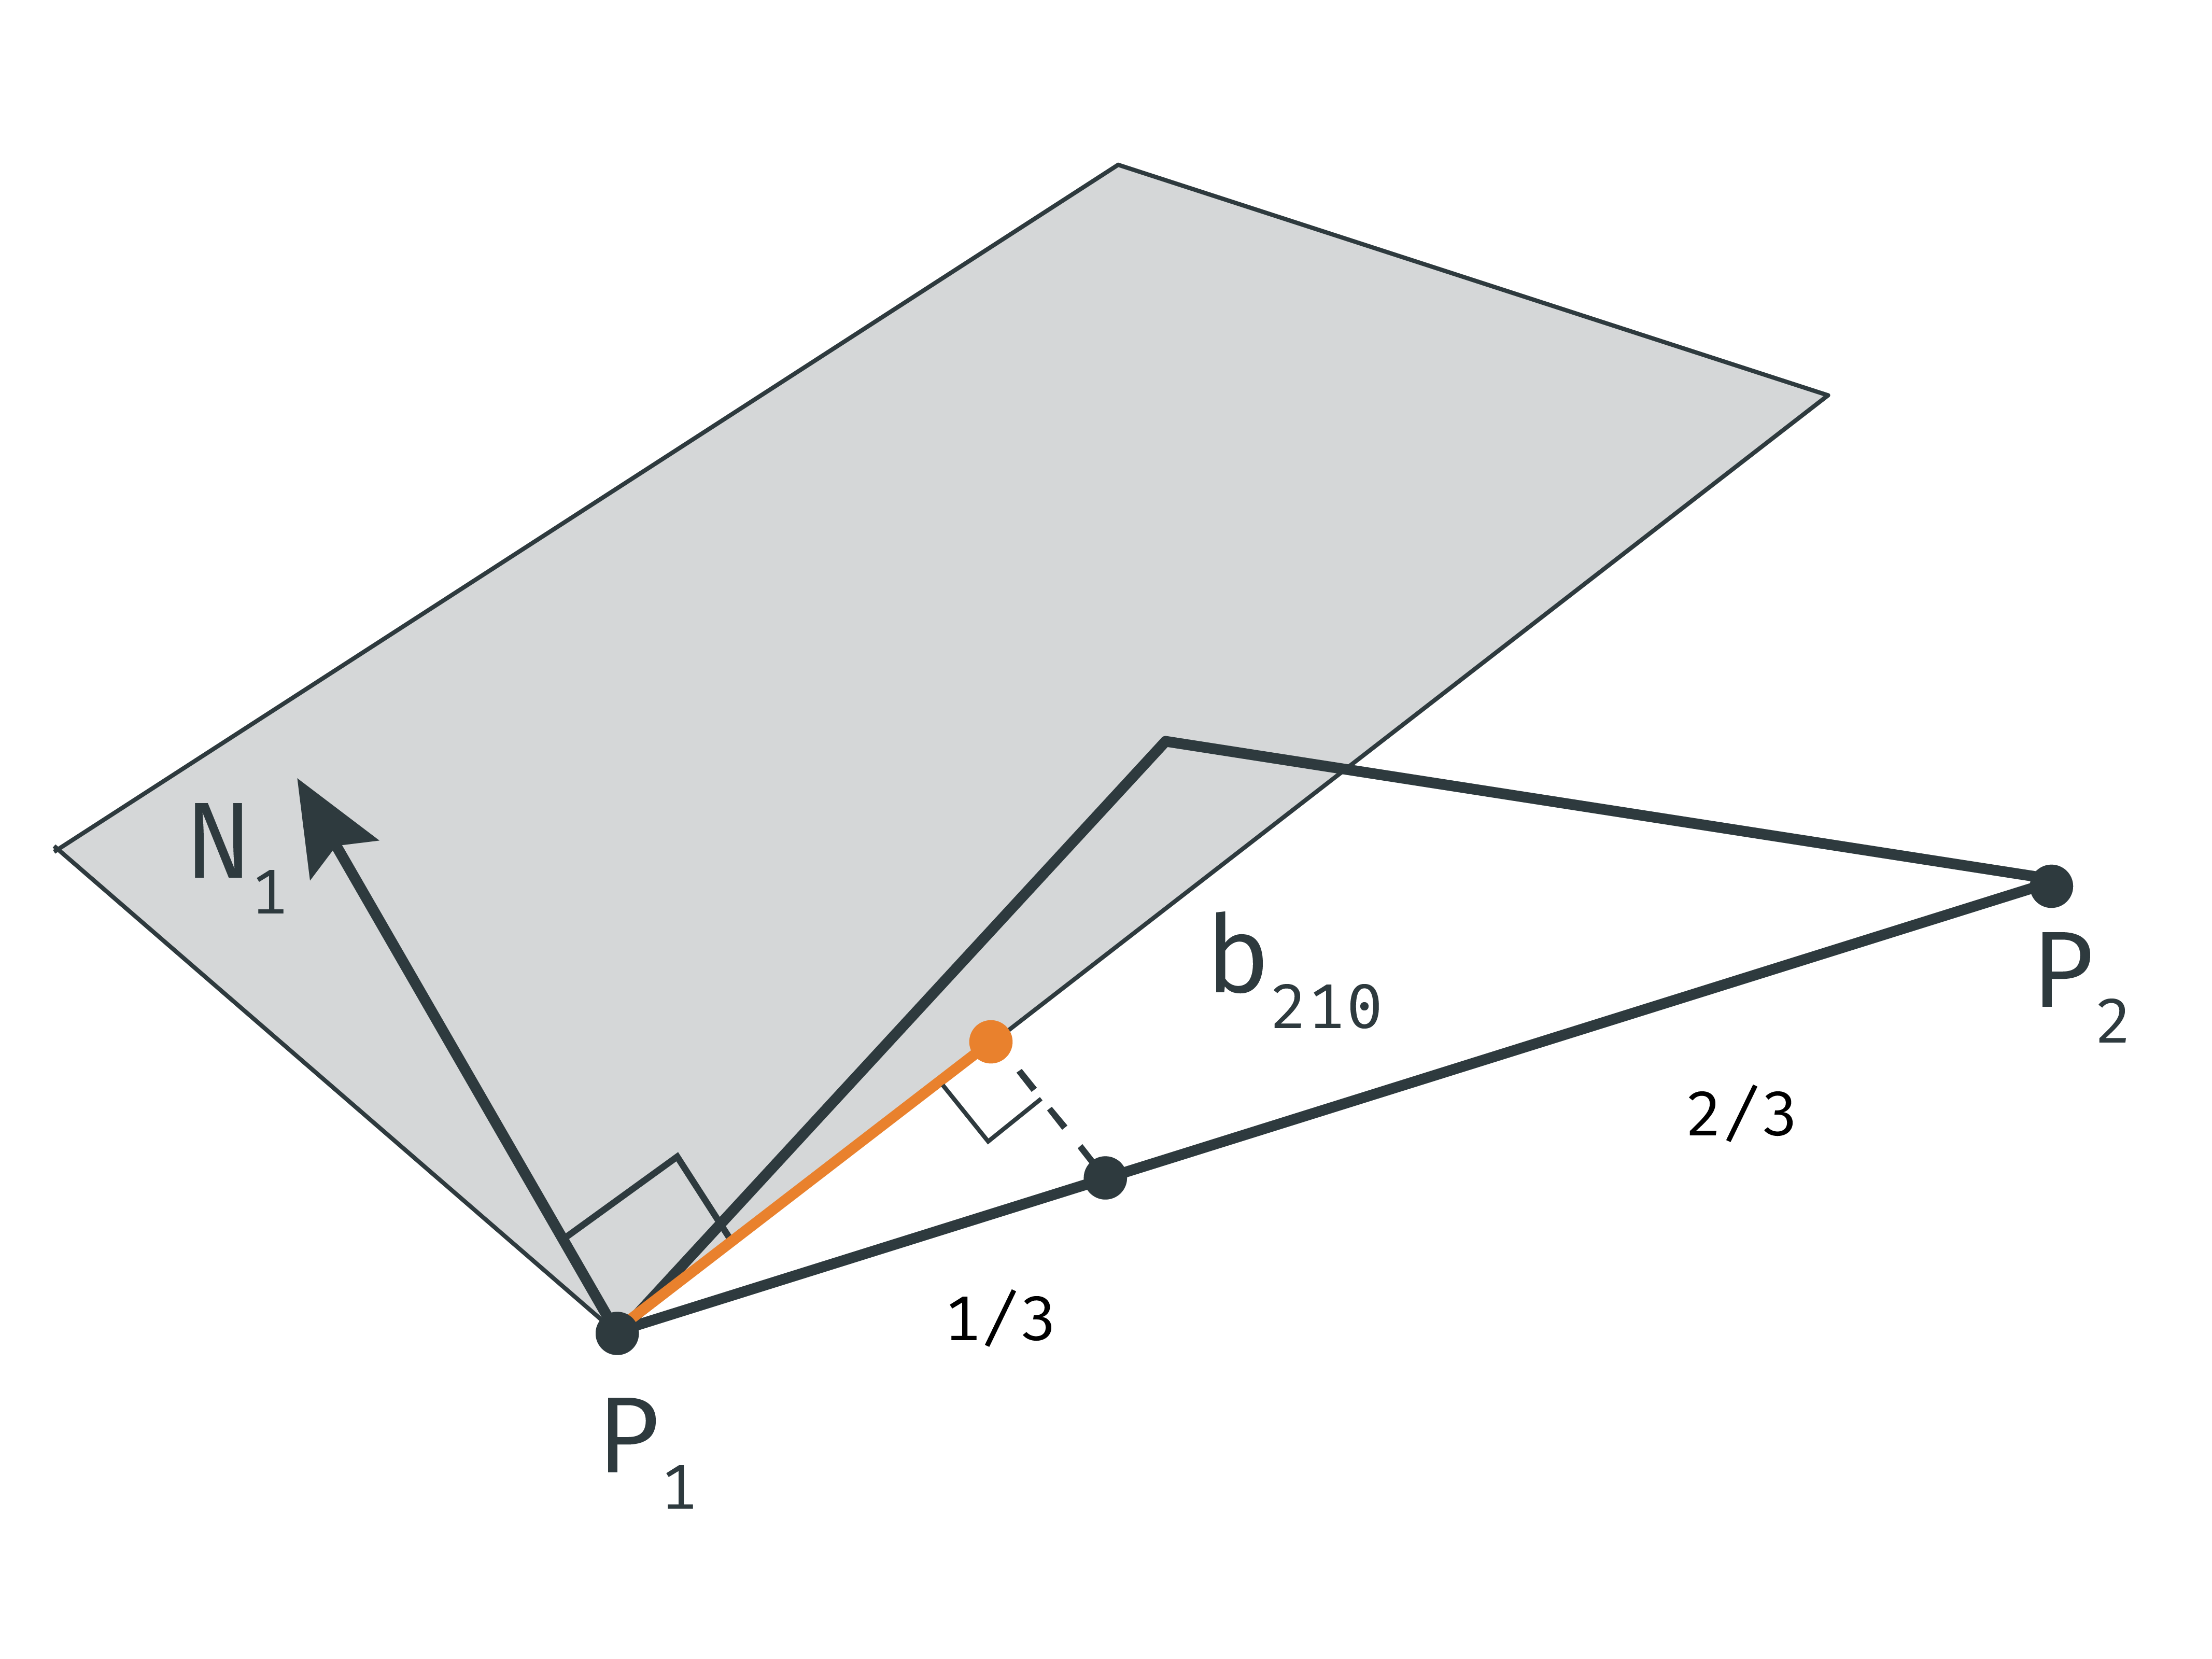
\includegraphics[width=\textwidth]{img/1_single/geometry_2.png}
				\small{Normal projection}
				\end{center}
			\end{column}
			\uncover<2>{
				\begin{column}{0.4\textwidth}
					\begin{equation*}
						A^2 + B^2 = C^2
					\end{equation*}
				\end{column}
			}
		\end{columns}
	\end{frame}

	\begin{frame}\frametitle{Geometry - step 3}
		\begin{columns}
			\begin{column}{0.6\textwidth}
				\begin{center}
				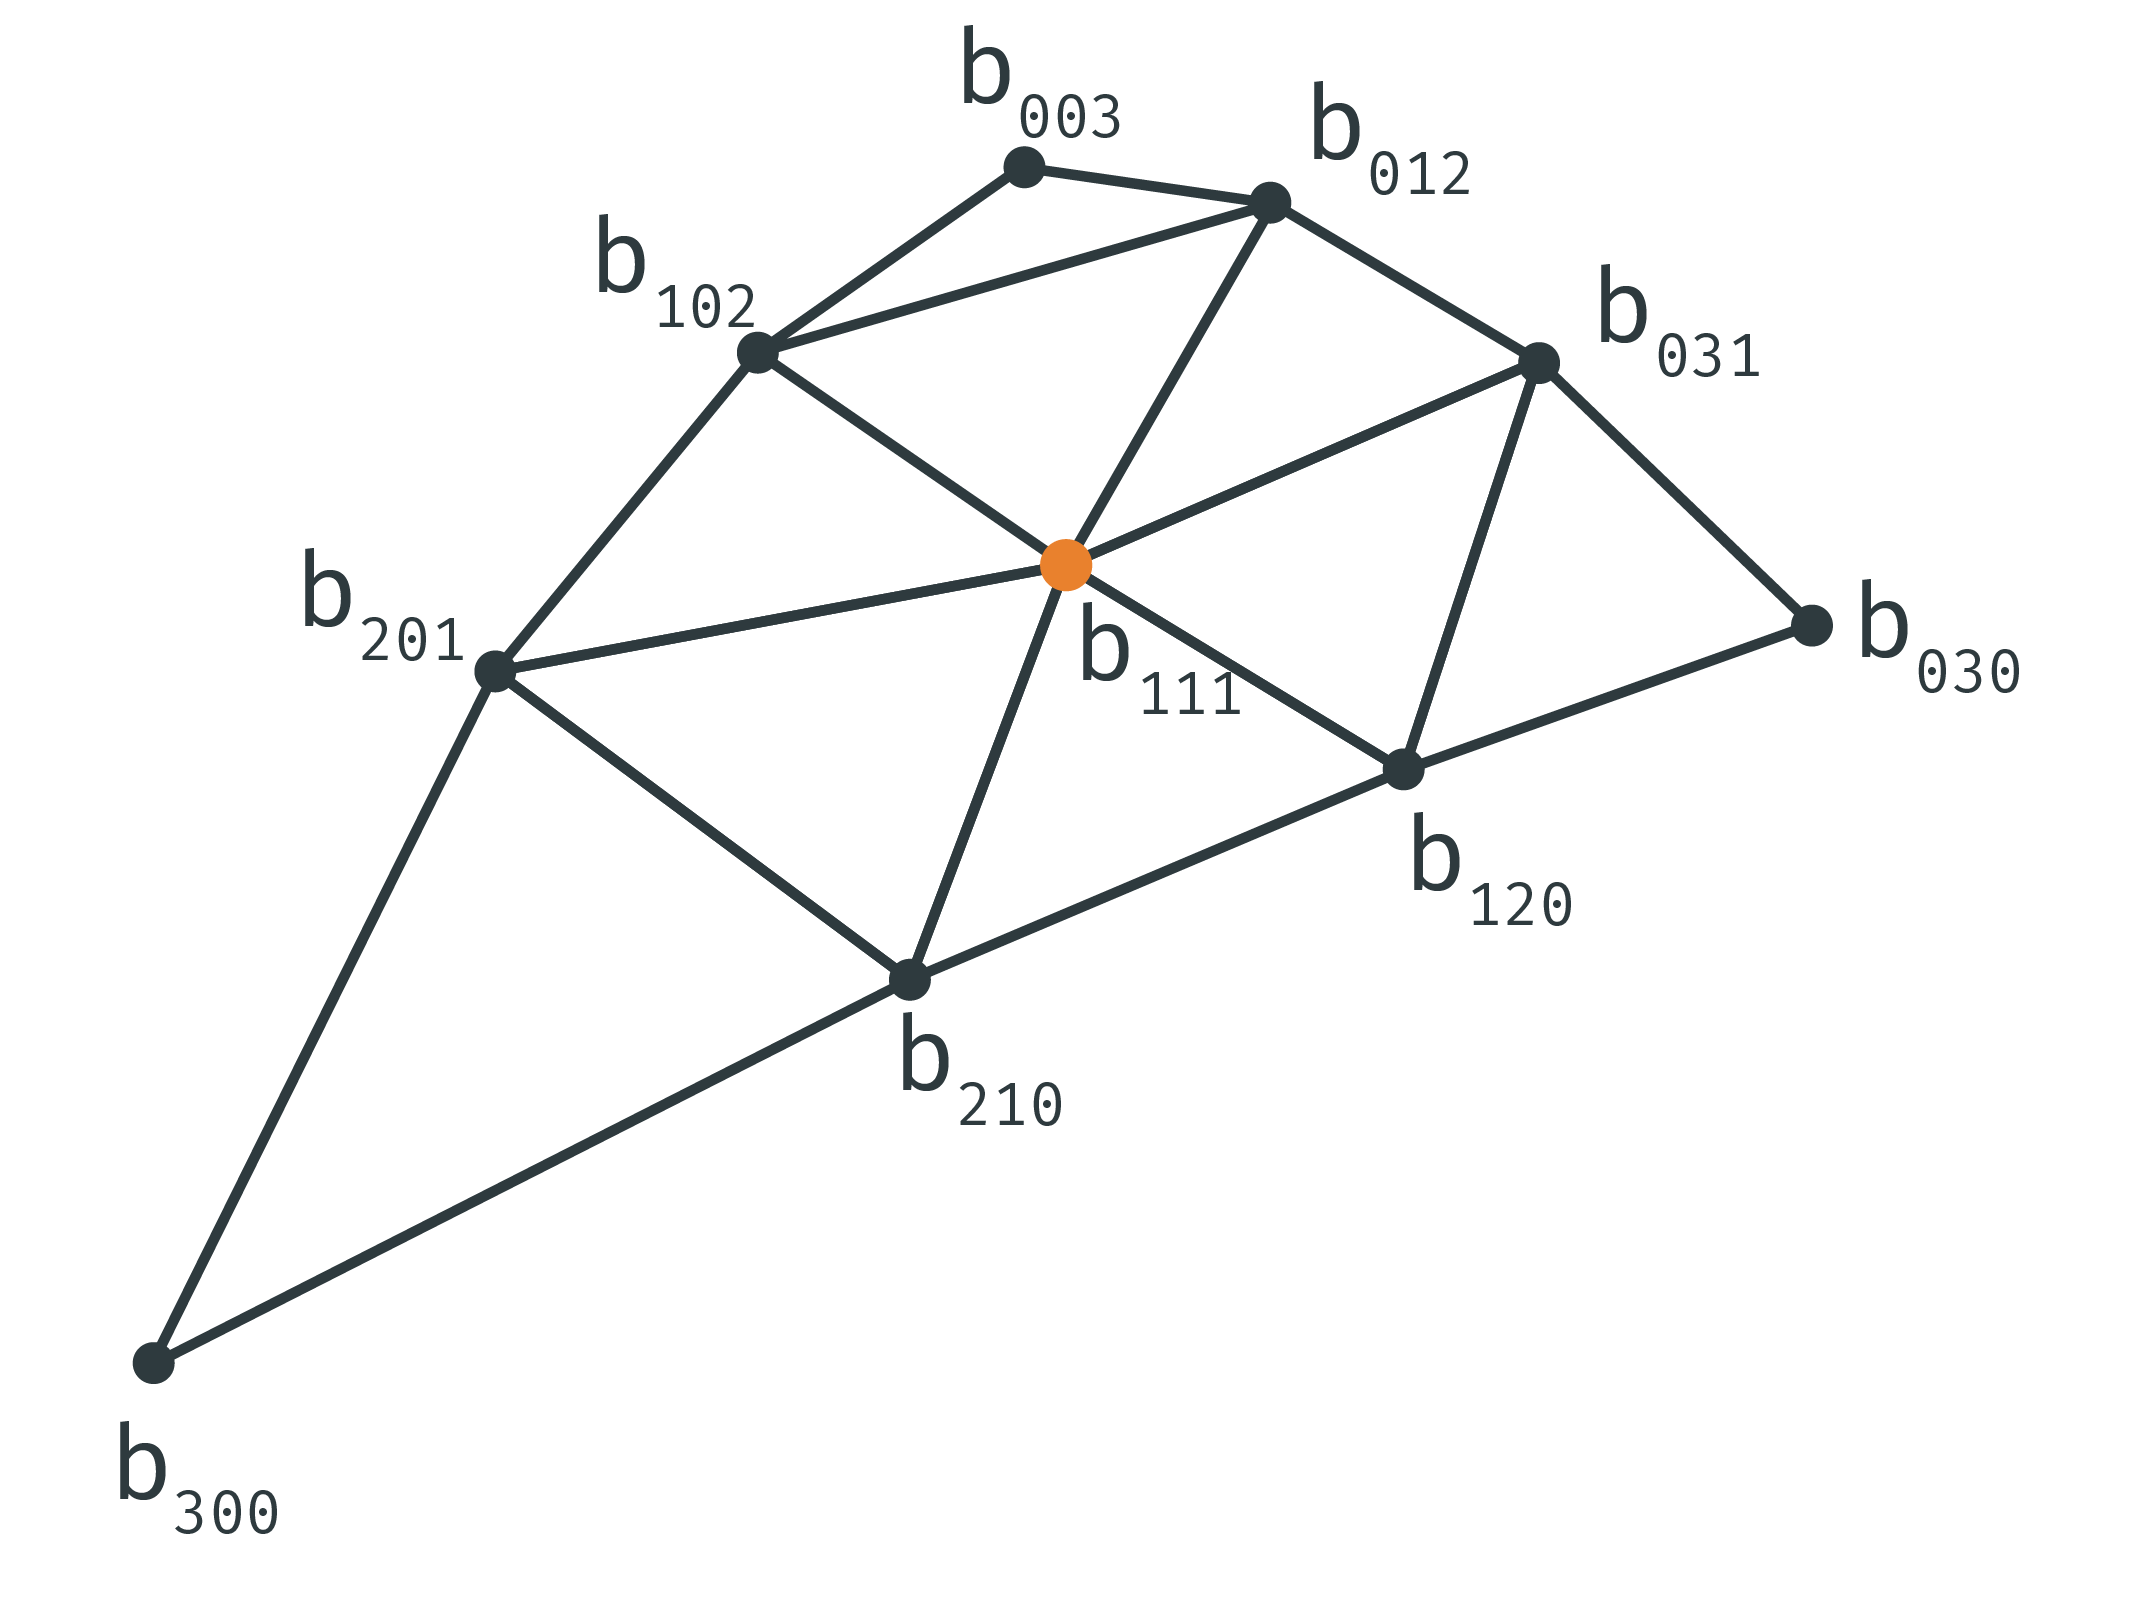
\includegraphics[width=\textwidth]{img/1_single/geometry_3.png}
				\small{Center control point}
				\end{center}
			\end{column}
			\uncover<2>{
				\begin{column}{0.4\textwidth}
					\begin{equation*}
						A^2 + B^2 = C^2
					\end{equation*}
				\end{column}
			}
		\end{columns}
	\end{frame}	

	\begin{frame}\frametitle{Geometry - result}
		% \todo[inline]{How do you create the PN triangle geometrically}
		\begin{columns}
			\begin{column}{0.6\textwidth}
				\begin{center}
				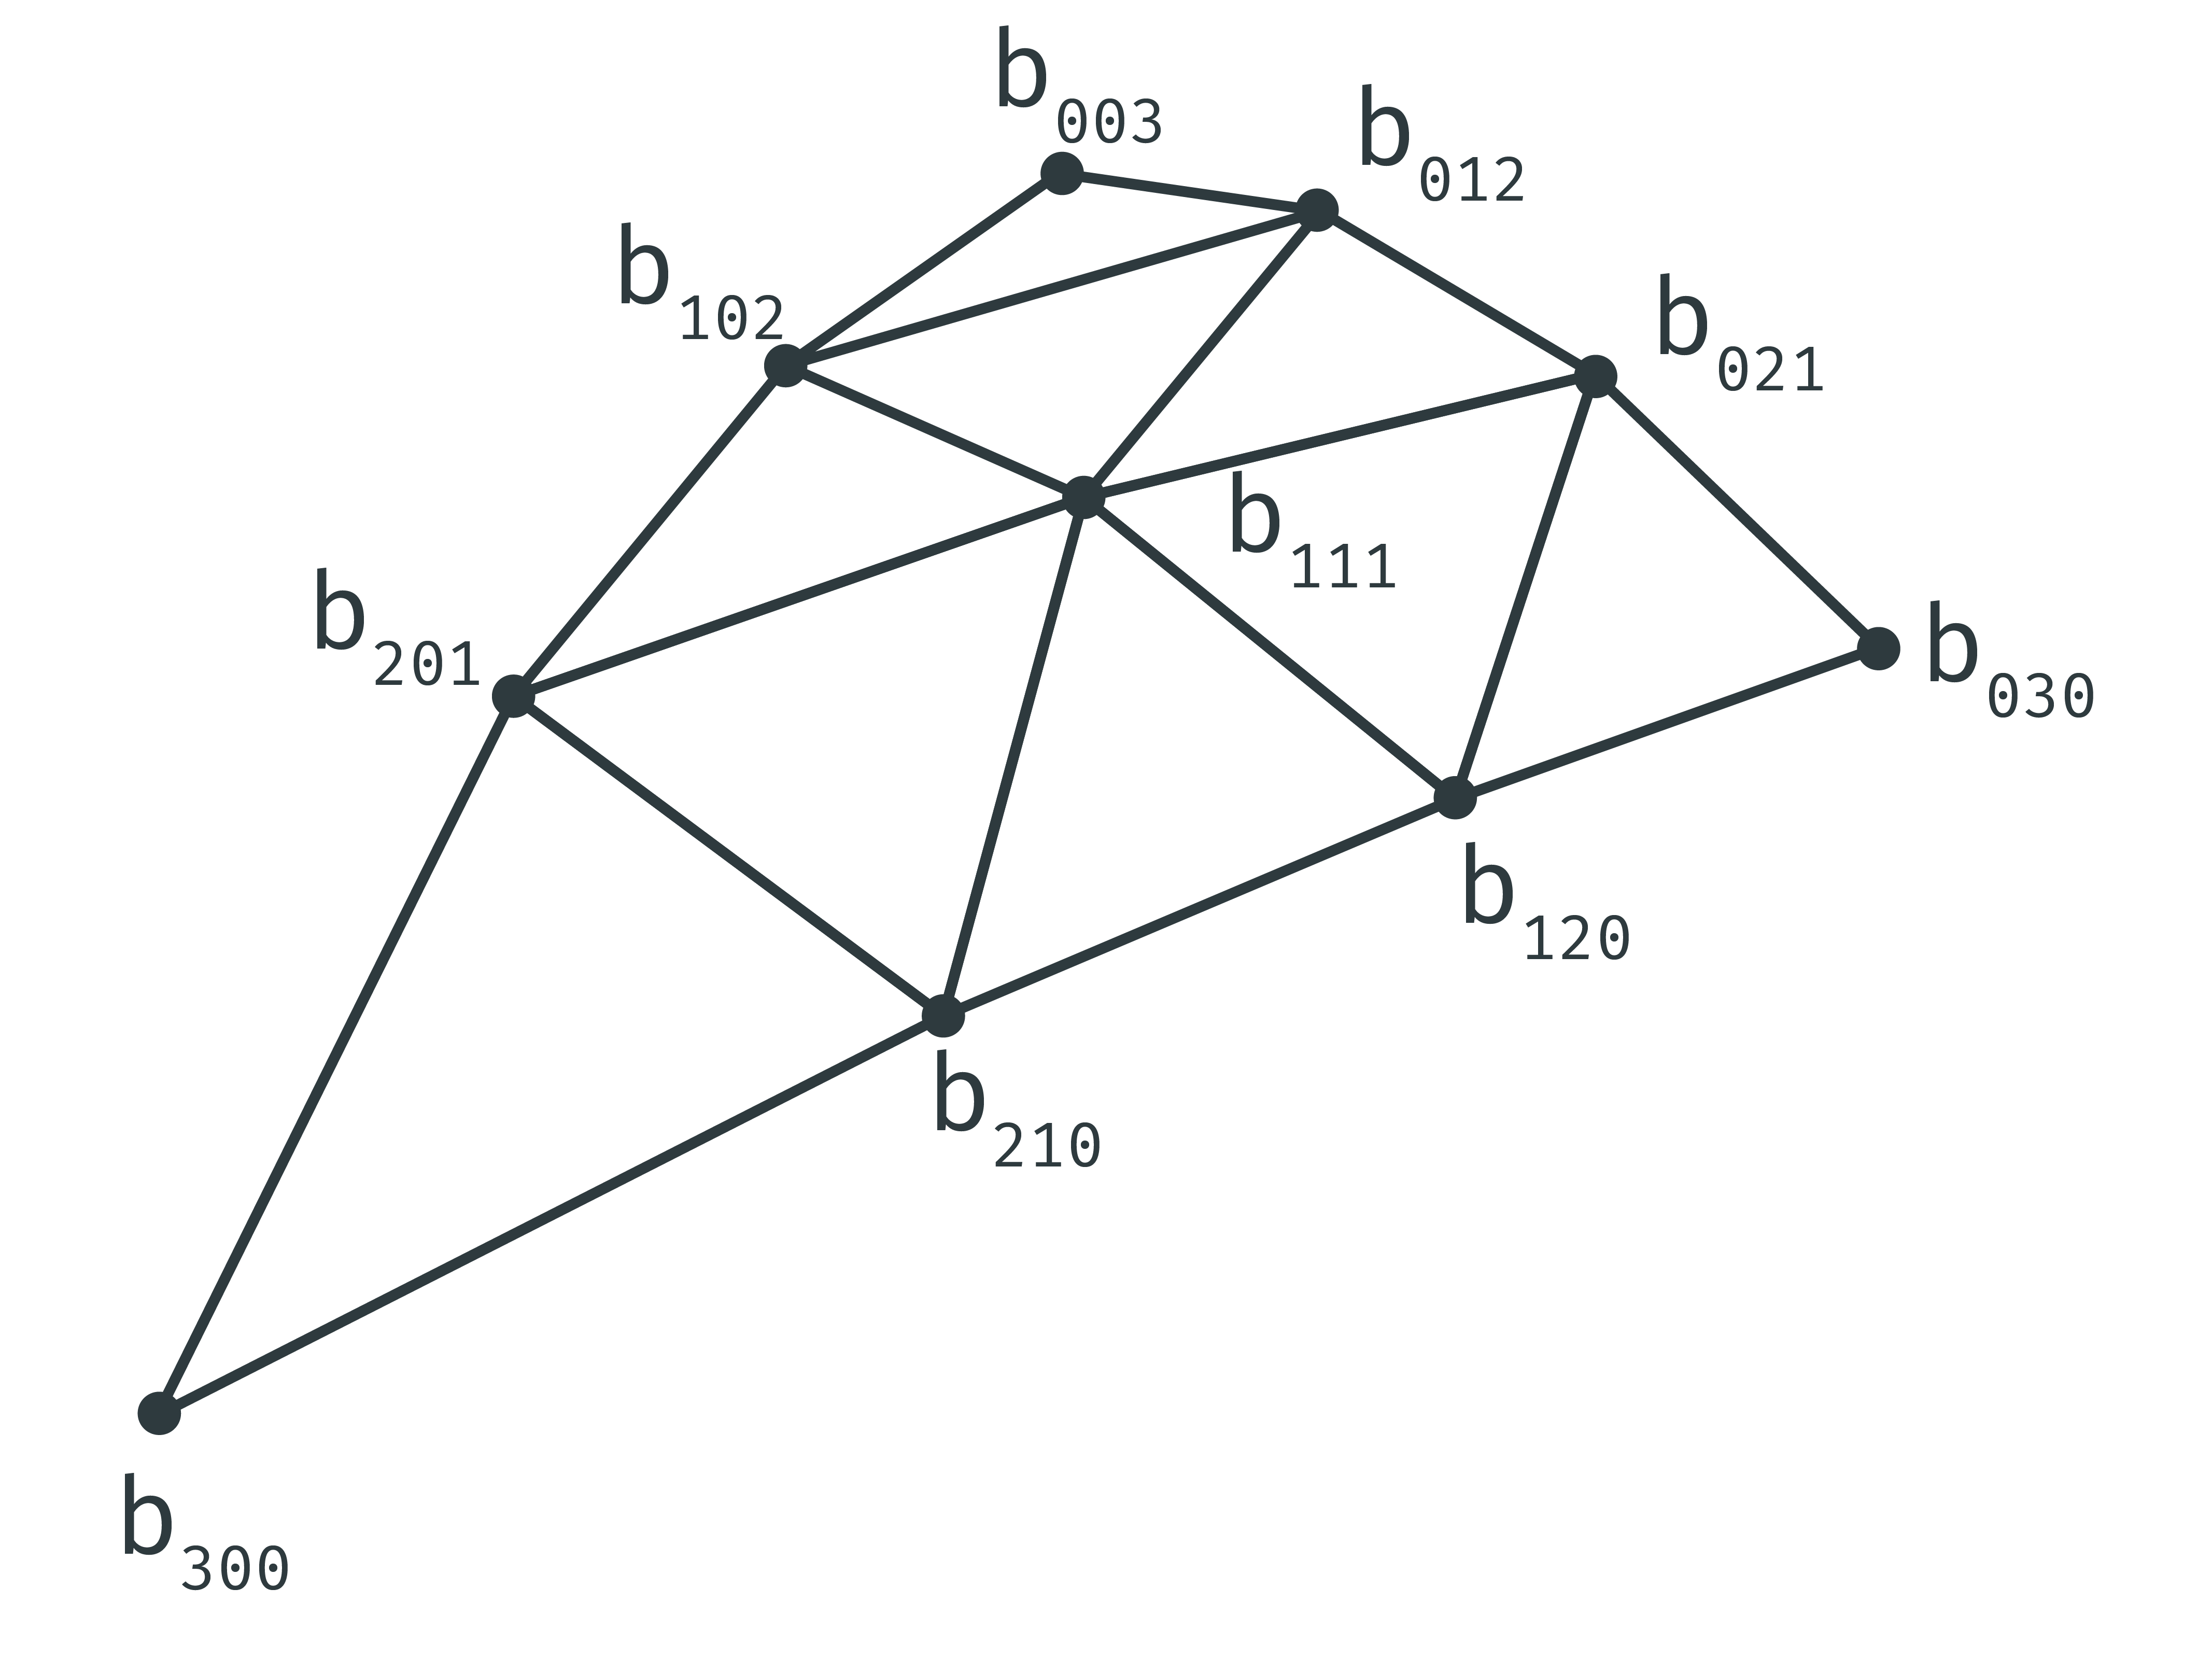
\includegraphics[width=\textwidth]{img/1_single/geometry_4.png}
				\end{center}	
			\end{column}
		\end{columns}
	\end{frame}

		\begin{frame}\frametitle{Normals}
		\begin{columns}
			\begin{column}{0.6\textwidth}
				\begin{center}
					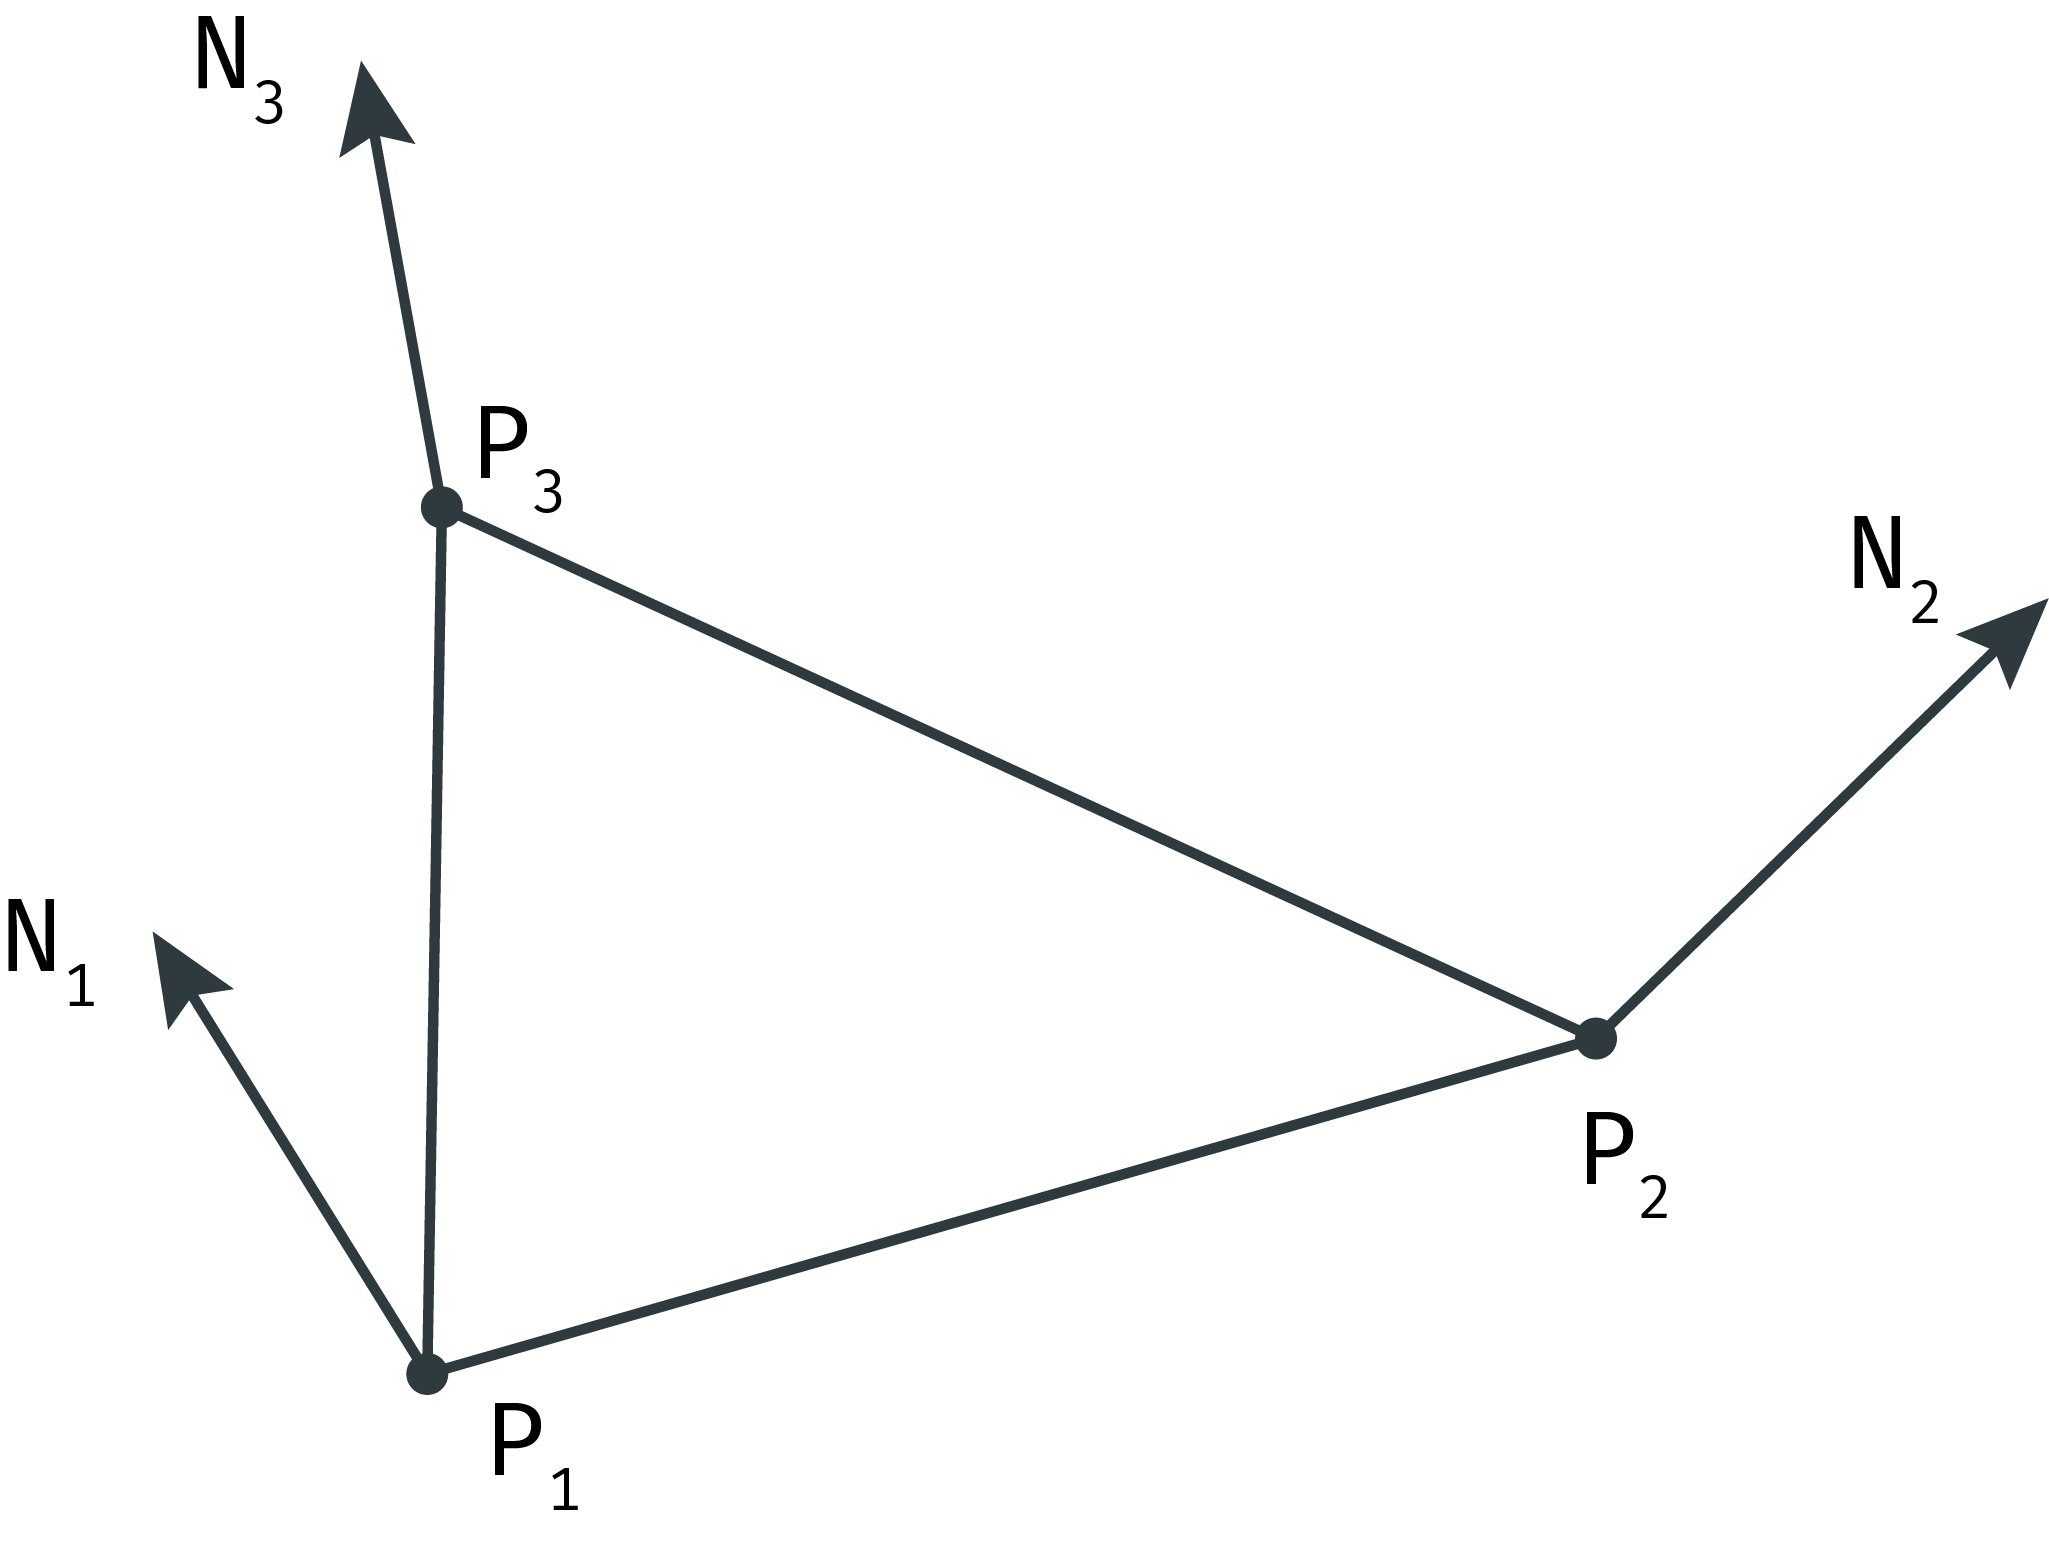
\includegraphics[width=\textwidth]{img/1_single/inputPrimitive.png}
					\small{Input primitive}
				\end{center}
			\end{column}
		\end{columns}
	\end{frame}

	\begin{frame}
		\frametitle{Normals}
		\begin{columns}
			\begin{column}{0.6\textwidth}
				\begin{center}
					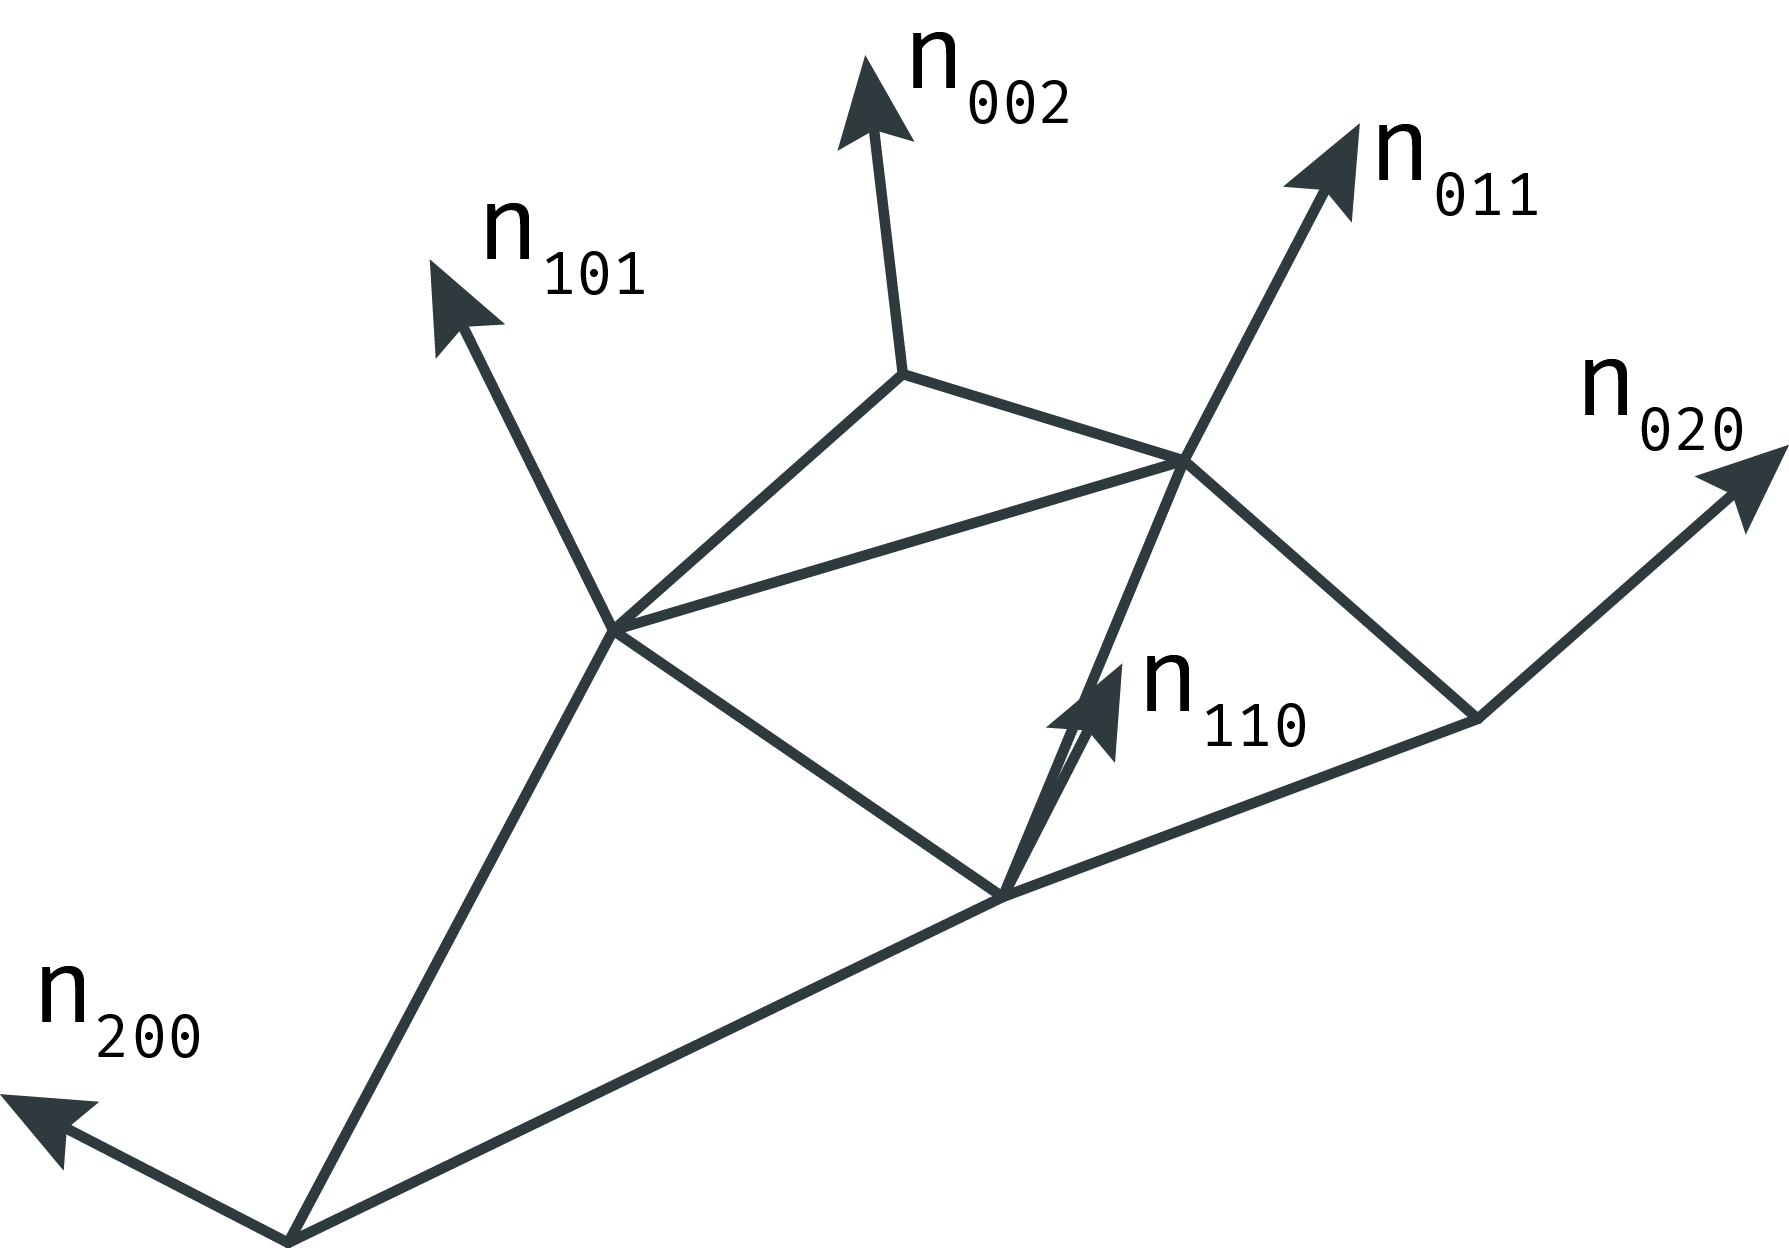
\includegraphics[width=\textwidth]{img/1_single/normals.png}
				\end{center}	
			\end{column}
			\uncover<2>{
				\begin{column}{0.4\textwidth}
					\begin{equation*}
						A^2 + B^2 = C^2
					\end{equation*}
				\end{column}
			}
		\end{columns}
	\end{frame}

	\begin{frame}\frametitle{Normals - theory}
		\begin{columns}
			\begin{column}{0.6\textwidth}
				\begin{center}
					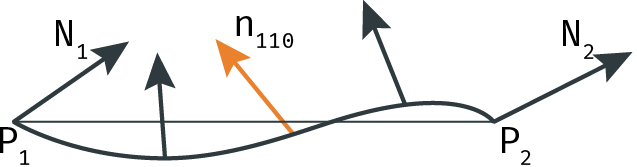
\includegraphics[width=\textwidth]{img/1_single/linearVsQuadraticNormals_linear.png}
					\small{Linear}
				\end{center}	
			\end{column}
		\end{columns}
		\pause
		\vspace{0.8cm}
		\begin{columns}
			\begin{column}{0.6\textwidth}
				\begin{center}
					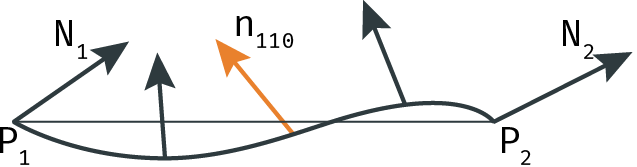
\includegraphics[width=\textwidth]{img/1_single/linearVsQuadraticNormals_quadratic.png}
					\small{Quadratic}
				\end{center}	
			\end{column}
		\end{columns}
	\end{frame}

	\begin{frame}\frametitle{Normals - theory}
		\begin{columns}
			\begin{column}{0.6\textwidth}
				\begin{center}
					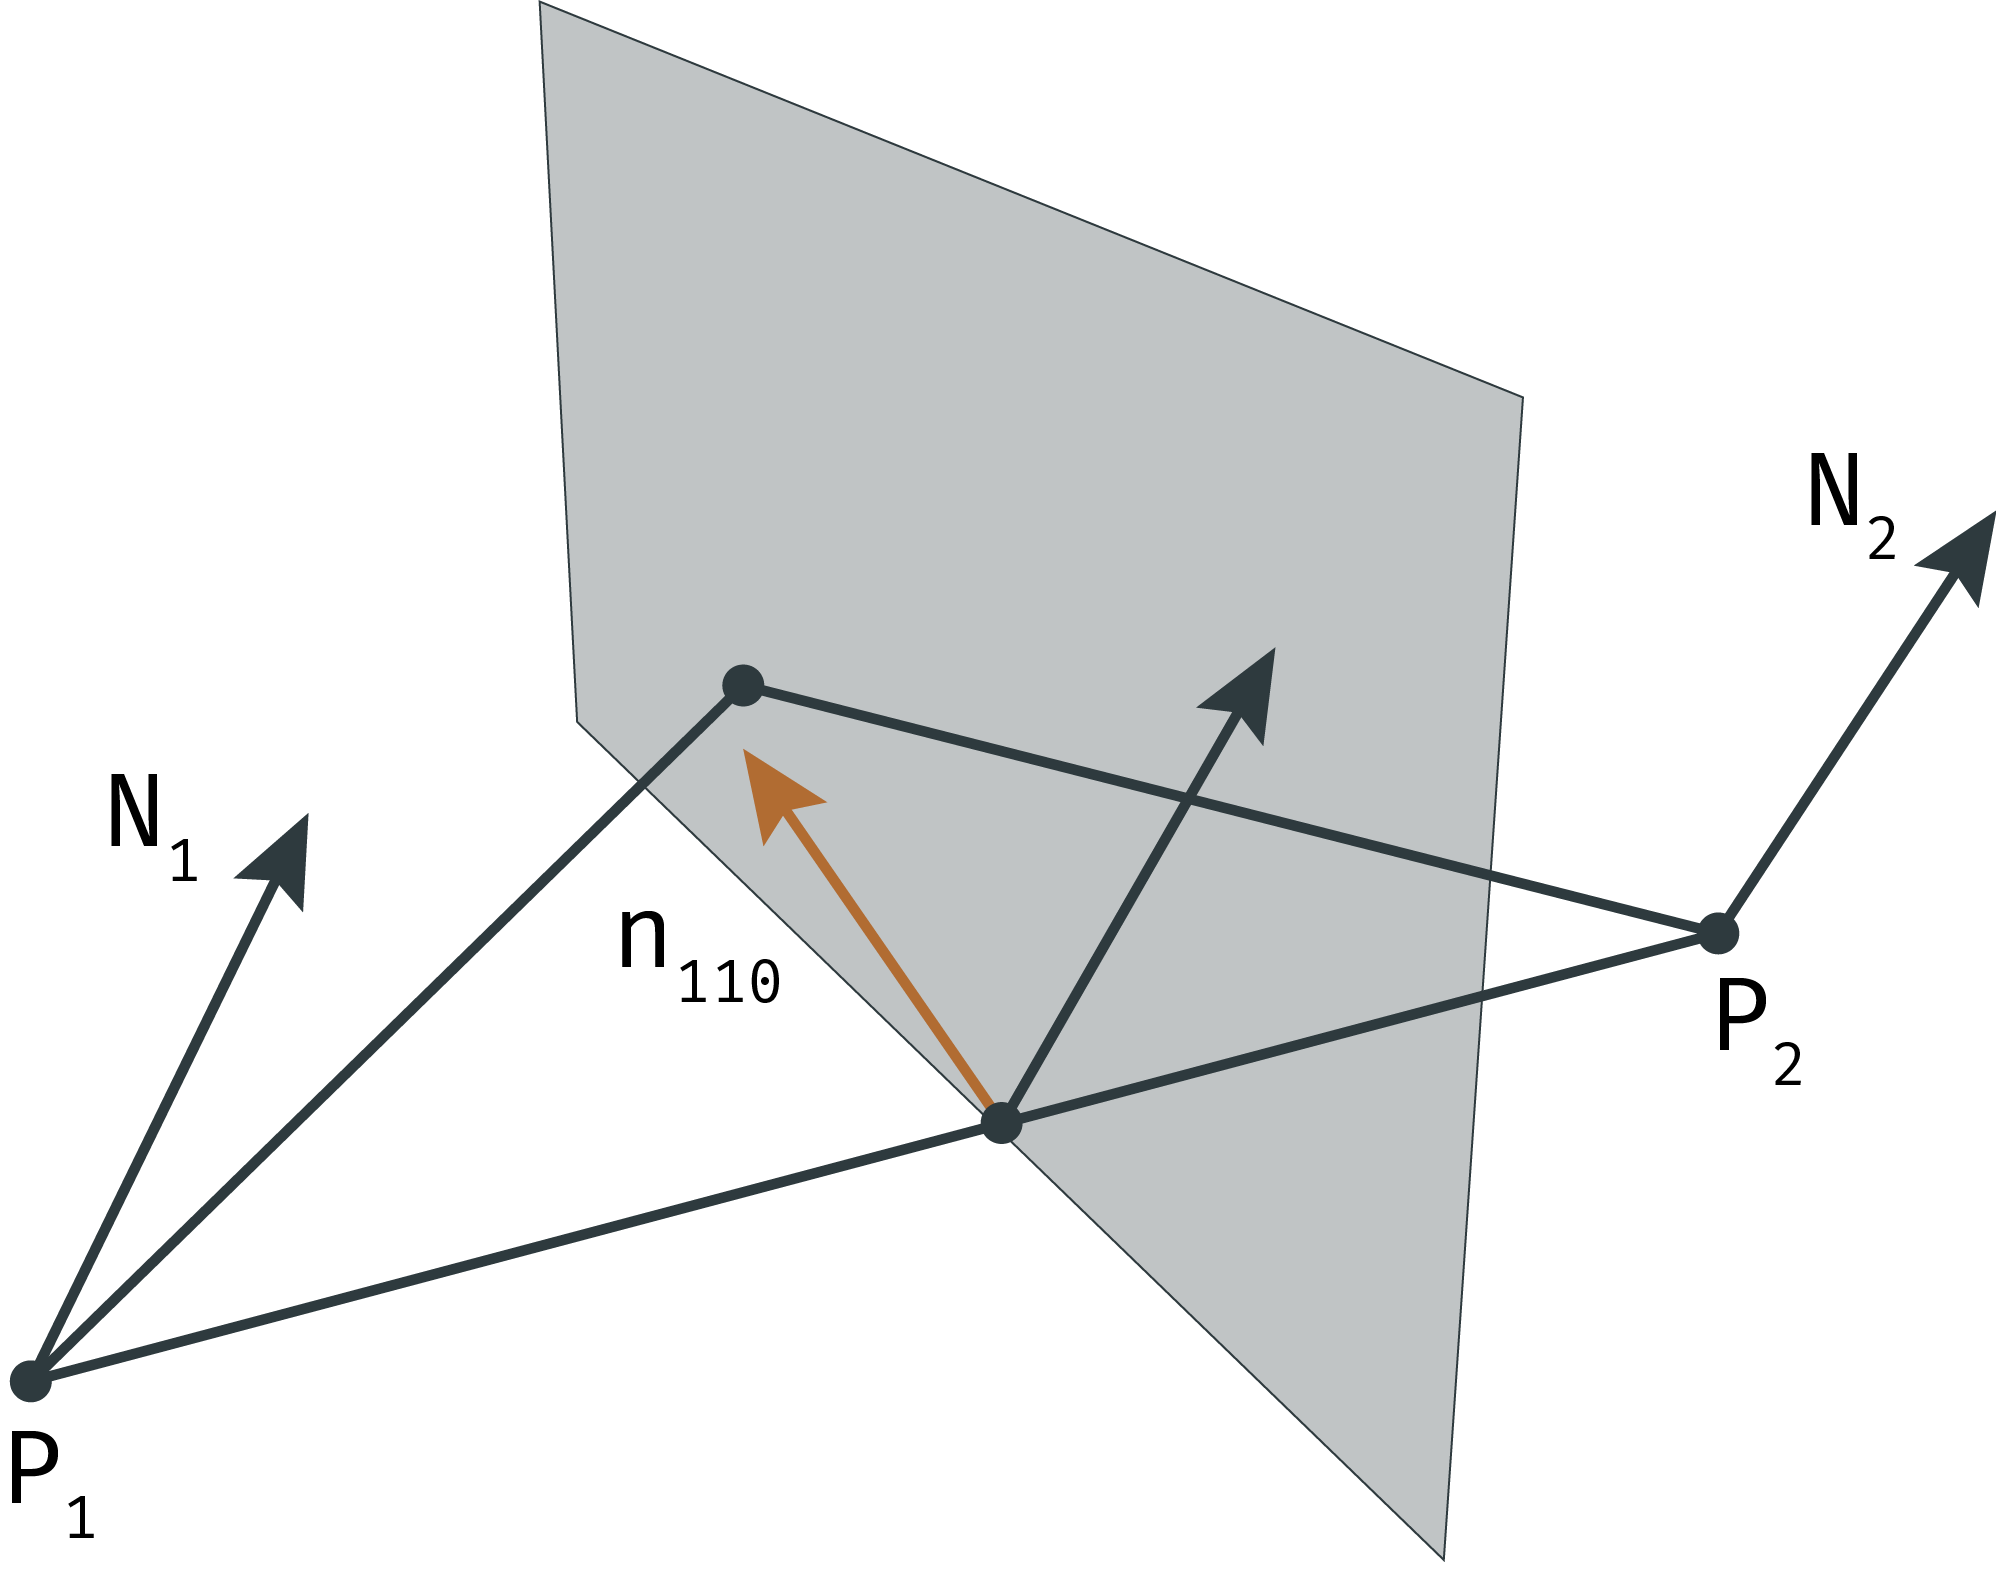
\includegraphics[width=\textwidth]{img/1_single/computingNormals.png}
				\end{center}
			\end{column}
			\uncover<2>{
				\begin{column}{0.4\textwidth}
					\begin{equation*}
						A^2 + B^2 = C^2
					\end{equation*}
				\end{column}
			}
		\end{columns}
	\end{frame}

	\begin{frame}\frametitle{Normals - result}
		\begin{columns}
			\begin{column}{0.4\textwidth}
			\begin{center}
					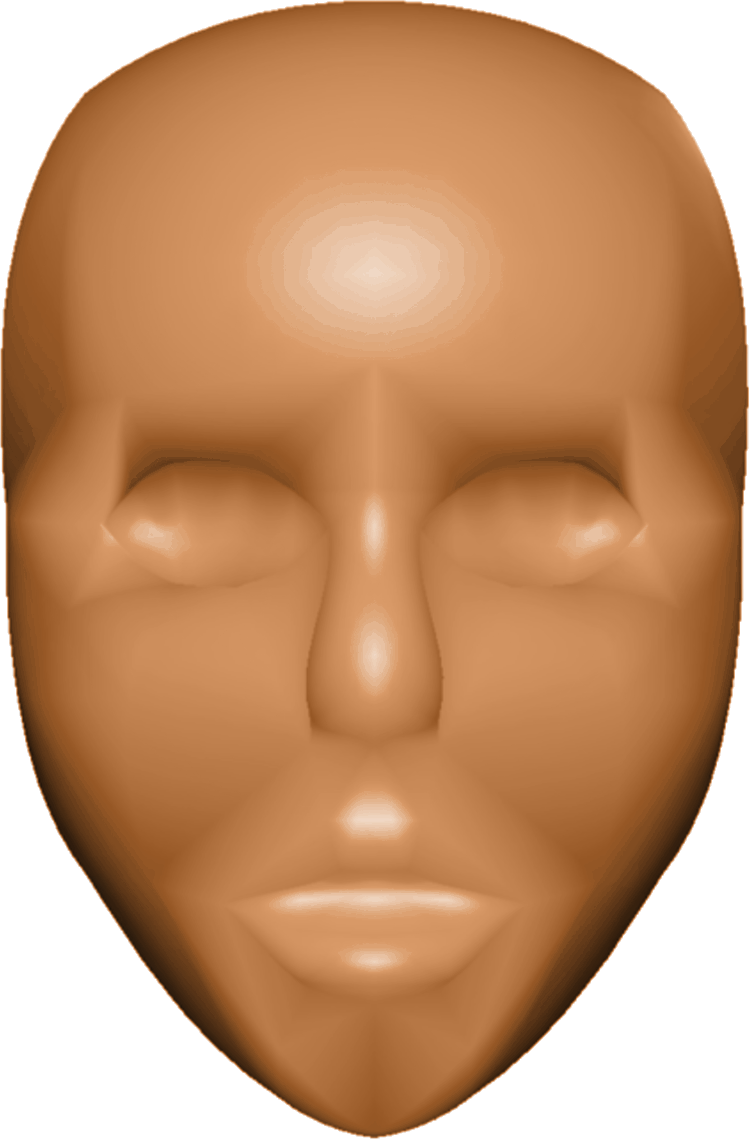
\includegraphics[width=\textwidth]{img/1_single/linearlyVaryingNormals.png}
					\small{Linear}
				\end{center}	
			\end{column}
			\begin{column}{0.4\textwidth}
			\begin{center}
					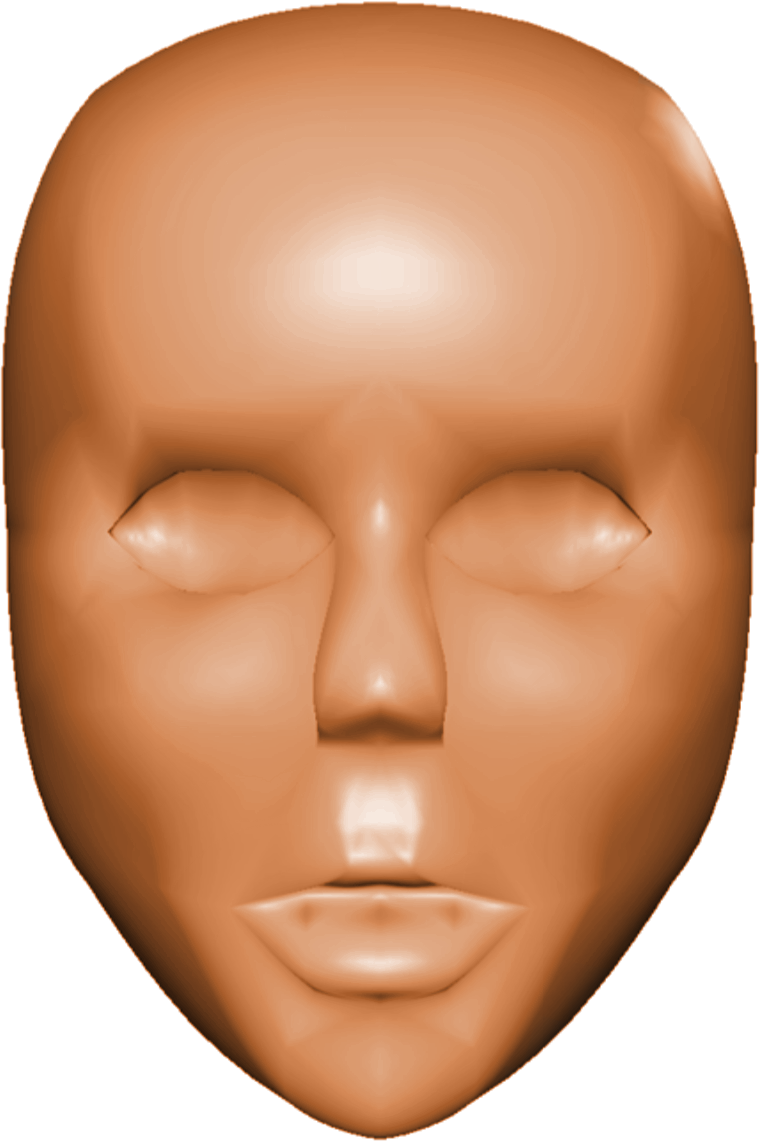
\includegraphics[width=\textwidth]{img/1_single/quadriticallyVaryingNormals.png}
					\small{Quadratic}
				\end{center}	
			\end{column}
		\end{columns}
	\end{frame}

	\begin{frame}
		\frametitle{Level Of Detail}
		\todo[inline]{Barycentric coordinates recap}
	\end{frame}	

	\begin{frame}
		\frametitle{Level Of Detail}
		\todo[inline]{LOD verhaal}
		\begin{columns}
			\begin{column}[b]{0.22\textwidth}
				\begin{center}
					
\includegraphics[width=\textwidth]{./img/1_single/lod_lod0.png}
					\small{0}
				\end{center}	
			\end{column}
			\begin{column}[b]{0.22\textwidth}
				\begin{center}
					
\includegraphics[width=\textwidth]{./img/1_single/lod_lod1.png}	
					\small{1}
				\end{center}	
			\end{column}
			\begin{column}[b]{0.22\textwidth}
				\begin{center}
					
\includegraphics[width=\textwidth]{./img/1_single/lod_lod2.png}	
					\small{2}
				\end{center}	
			\end{column}
			\begin{column}[b]{0.22\textwidth}
				\begin{center}
					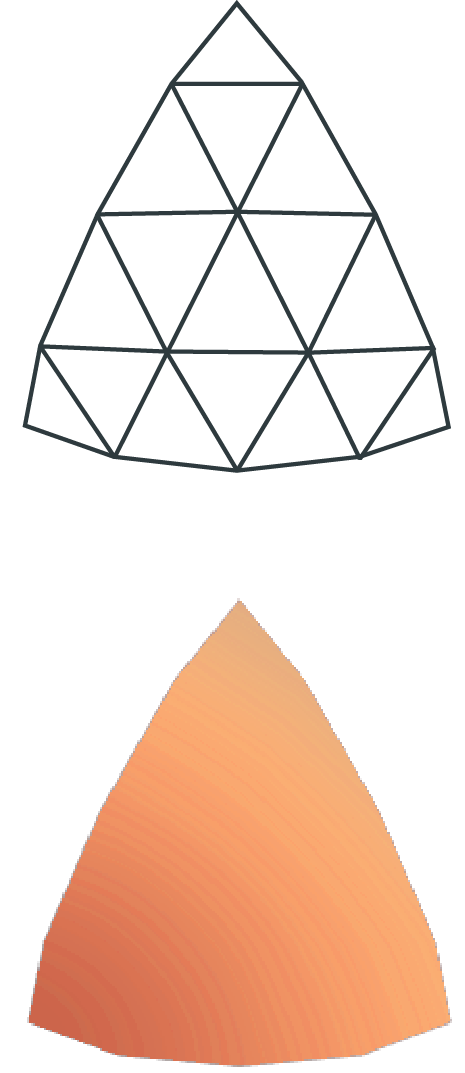
\includegraphics[width=\textwidth]{./img/1_single/lod_lod3.png}	
					\small{3}
				\end{center}	
			\end{column}
		\end{columns}
	\end{frame}	

	\begin{frame}
		\frametitle{Construction}
		\todo[inline]{The steps. Recap of everything construct geometry and normals and evaluate less (low lod) or more points (high lod)}
	\end{frame}	

	\section{A Triangle Mesh}
	% !TEX root = presentation.tex
% { % all template changes are local to this group.
%     \begin{frame}[plain]
%         \begin{tikzpicture}[remember picture,overlay]
%             \node[at=(current page.center)] {
%                 \includegraphics[width=\paperwidth]{./img/03_tomb-raider-underworld}
%             };
%         \end{tikzpicture}
%      \end{frame}
% }


\begin{frame}\frametitle{Properties}
	\begin{quote}
		``PN triangles should not deviate too much from the original triangle to preserve the shape and avoid interference with other curved triangles."
		\footnote{\citeauthor{vlachos2001curved}}
	\end{quote}
\end{frame}

\begin{frame}\frametitle{Continuity}	
	PN triangles have:\footnote{\citeauthor{jiao2005parallel}}
	\begin{itemize}
		\item $C^1$ continuity in the vertex points
		\item $C^0$ continuity everywhere else
	\end{itemize}
\end{frame}

\begin{frame}\frametitle{Sharp Edges}
	\begin{columns}
		\begin{column}[b]{0.22\textwidth}
			\begin{center}
				
\includegraphics[width=\textwidth]{./img/2_mesh/bluntAxeMesh.png}
				\small{mesh}
			\end{center}	
		\end{column}
		\begin{column}[b]{0.22\textwidth}
			\begin{center}
				
\includegraphics[width=\textwidth]{./img/2_mesh/bluntAxeShaded.png}
				\small{blunt}
			\end{center}	
		\end{column}
		\begin{column}[b]{0.22\textwidth}
			\begin{center}
				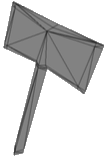
\includegraphics[width=\textwidth]{./img/2_mesh/sharpAxeMesh.png}
				\small{mesh}
			\end{center}	
		\end{column}
		\begin{column}[b]{0.22\textwidth}
			\begin{center}
				
\includegraphics[width=\textwidth]{./img/2_mesh/sharpAxeShaded.png}
				\small{sharp}
			\end{center}	
		\end{column}
	\end{columns}
\end{frame}	

\begin{frame}\frametitle{Separate Normals}
	\begin{columns}
		\begin{column}{0.4\textwidth}
		\begin{center}
				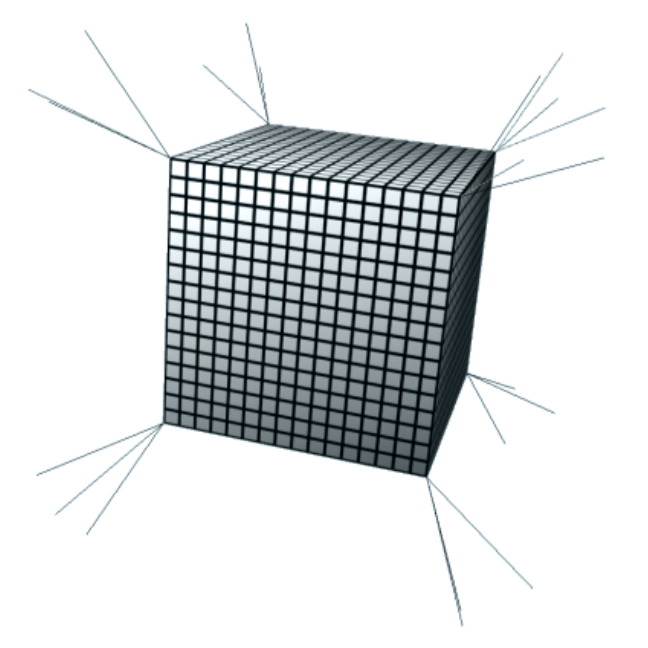
\includegraphics[width=\textwidth]{img/2_mesh/cracksNormals.png}
				\small{normals}
			\end{center}	
		\end{column}
		\begin{column}{0.4\textwidth}
		\begin{center}
				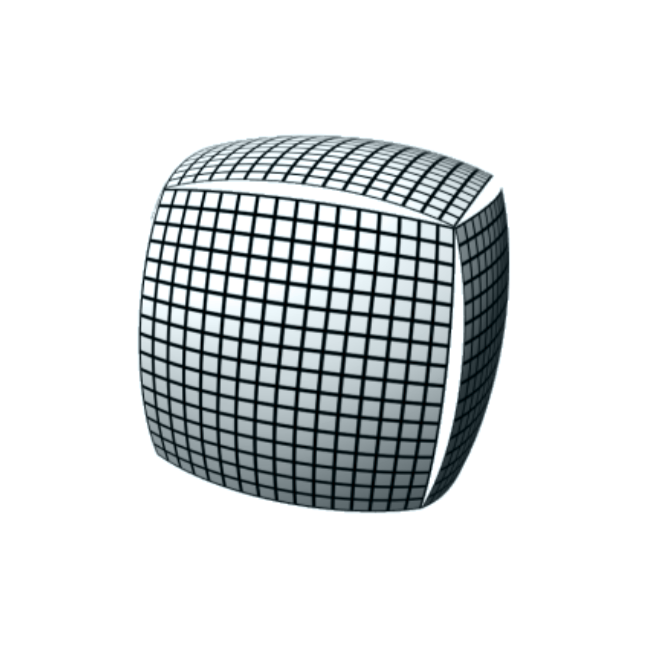
\includegraphics[width=\textwidth]{img/2_mesh/cracks.png}
				\small{cracks}
			\end{center}	
		\end{column}
	\end{columns}
\end{frame}


	\section{Graphics Pipeline}
	% !TEX root = presentation.tex
% { % all template changes are local to this group.
%     \begin{frame}[plain]
%         \begin{tikzpicture}[remember picture,overlay]
%             \node[at=(current page.center)] {
%                 \includegraphics[width=\paperwidth]{./img/03_tomb-raider-underworld}
%             };
%         \end{tikzpicture}
%      \end{frame}
% }


	\begin{frame}\frametitle{Hardware - Pipelines}
		\begin{columns}
			\begin{column}{0.9\textwidth}
				\begin{center}
					
\includegraphics[width=\textwidth]{img/3_pipeline/pipelineDifferences_oldOpenGL.png}
					\small{2001}
				\end{center}	
			\end{column}
		\end{columns}
		\pause
		\vspace{0.8cm}
		\begin{columns}
			\begin{column}{0.9\textwidth}
				\begin{center}
					
\includegraphics[width=\textwidth]{img/3_pipeline/pipelineDifferences_newOpenGL.png}
					\small{2015}
				\end{center}	
			\end{column}
		\end{columns}
	\end{frame}

% \begin{frame}
% 	\frametitle{Hardware - Pipelines}
%     \todo[inline]{Hoe zou je het nu kunnen implementeren? Plus pipeline}
% \end{frame}

	\section{Conclusion}
	% !TEX root = presentation.tex

\plain{	
    \begin{center}
    	\LARGE{questions?}
    \end{center}		
	\begin{columns}
		\begin{column}[b]{.5\textwidth}
			\begin{center}
				
\includegraphics[
					width=\textwidth, 
					height=0.7\textheight,
					keepaspectratio=true
				]{./img/4_conclusion/finalresultNoPN.png}

				\small{triangles}
			\end{center}
		\end{column}
		\begin{column}[b]{.5\textwidth}
			\begin{center}
				
\includegraphics[
					width=\textwidth, 
					height=0.7\textheight,
					keepaspectratio=true
				]{./img/4_conclusion/finalResultPN.png}								

				\small{pn triangles}
			\end{center}
		\end{column}
	\end{columns}
}

	\section{References}
	% !TEX root = presentation.tex

\begin{frame}\frametitle{References}
	\printbibliography[heading=none]
	\note{~}
\end{frame}


\end{document}